% ============================================================
%  Forces and Motion — Lesson Booklet (one section per lesson: A Reading · B Theory · C Practice · D Above level)
%  Years 7–8  |  Victorian Curriculum F–10 Version 2.0
%  Compile with: xelatex, three times (see CLAUDE.md) --- fill.py does this and sizes the answer boxes
%
%  TWO BUILDS FROM THIS ONE SOURCE (the Ch3G-L / Trebuchet pattern)
%    Forces_Motion_Lesson_Booklet_Yr7_8.tex          student copy --- no answers
%    Forces_Motion_Lesson_Booklet_Yr7_8_Teacher.tex  teacher copy --- defines
%        \teacheranswers (every \defans, read from teacher-answers/L01.tex ...
%        L14.tex, plus \teacherappendix) and then \input's this file, so every
%        box, cell, drawing space and graph prints its model answer in red.
%  The teacher wrapper, teacher-answers/ and the teacher PDF are gitignored:
%  answer keys never ship as a plain file (ROADMAP.md, "Staff material").
%  Keep this file free of answers. A key missing from the wrapper prints
%  ??key?? in the teacher copy, so grep the teacher PDF for "??" after a build.
%
%  Every answer-bearing piece of furniture carries a key: \abox{key}{h} (ruled
%  writing box), \wbox{key}{h} (plain box for calculations), \rcqk{key}{q}{h}
%  (comprehension Cn), \cell{key} (write-in table cell), \drawk{key}{h}{caption}
%  and \graphgrid{key}{h}. Keys were set from the printed numbering on
%  30 Oct 2026 (6.t3b = Task 6.3(b), 6.x9 = Extension 6.9, 6.c2 = C2,
%  6.wd1a = We do 6.1(a), 6.pred = prediction, 6.v3 = vocab row 3,
%  6.res-r2c3 = results table row 2 column 3) and are literal from then on:
%  renumbering the booklet never moves an answer. New furniture needs a new key.
%
%  Both copies paginate identically: answers sit inside fixed-height boxes and
%  cells. The teacher build reads the STUDENT page-fill file (.abx) and never
%  writes one, so build the student copy (and run fill.py) first. Both builds
%  log every key with its page and printed label to <jobname>.akp; the two
%  files must agree page for page (tools/forces_solutions.py checks this).
% ============================================================
\documentclass[11pt,a5paper,twoside]{article}
\newcommand{\unitname}{Forces and Motion}\newcommand{\unitcaps}{FORCES AND MOTION}

% ── Student / teacher switch ─────────────────────────────────────────────────
% The teacher wrapper defines \teacheranswers (every \defans) before \input-ing
% this file. Without it this is the student copy and every answer is blank.
\newif\ifteacher
\makeatletter
\newcommand{\defans}[2]{\@namedef{kans@#1}{#2}}
\newcommand{\getans}[1]{\@ifundefined{kans@#1}{\textbf{??#1??}}{\@nameuse{kans@#1}}}
\newcommand{\hasans}[1]{\@ifundefined{kans@#1}{\@secondoftwo}{\@firstoftwo}}
\makeatother
\ifdefined\teacheranswers \teachertrue \teacheranswers \fi
% Page-fill files always use the student copy's name, so the teacher build
% reads the student layout and never writes its own.
\providecommand\abbase{\jobname}

% ── Fonts (compile with XeLaTeX) ────────────────────────────────────────────
\usepackage{fontspec}
% Bundled fonts (in ./fonts/) so the document compiles anywhere with XeLaTeX/LuaLaTeX
\setmainfont{Lato}[                   % body — humanist sans (stands in for deck's Inter)
  Path=../fonts/, Extension=.ttf, Ligatures=TeX,
  UprightFont=Lato-Regular, ItalicFont=Lato-Italic,
  BoldFont=Lato-Bold, BoldItalicFont=Lato-BoldItalic ]
\newfontfamily\headingfont{Poppins}[  % display/headings — matches the slide decks
  Path=../fonts/, Extension=.ttf, Ligatures=TeX,
  UprightFont=Poppins-Regular, ItalicFont=Poppins-Italic,
  BoldFont=Poppins-Bold, BoldItalicFont=Poppins-BoldItalic ]
\setlength{\headheight}{22pt}

\usepackage[protrusion=true,expansion=false]{microtype}
\usepackage[a5paper, inner=17mm, outer=13mm, top=19mm, bottom=17mm, headheight=14pt, headsep=4mm, footskip=8mm]{geometry}
\usepackage{xcolor}
\usepackage{tikz}
\usetikzlibrary{arrows.meta, shapes.geometric, calc, positioning, decorations.pathreplacing}
\usepackage{tcolorbox}
\tcbuselibrary{skins, breakable, raster}
\usepackage{fancyhdr}
\usepackage{titlesec}
\usepackage{enumitem}
\usepackage{booktabs}
\usepackage{tabularx}
\usepackage{array}
\usepackage{colortbl}
\usepackage{multicol}
\usepackage{amsmath}
\usepackage{needspace}
% TikZ diagram macros are embedded below (just before \begin{document}) for easy editing.
\usepackage{longtable}
\usepackage{graphicx}
\usepackage{lastpage}
\usepackage{calc}
\usepackage{mdframed}
\usepackage{setspace}
\usepackage{ragged2e}
% PDF bookmarks: one per lesson (made in \sectiondiv) plus the cover and
% contents, and links from the contents table to each lesson.
% implicit=false: hyperref adds no anchors of its own (an anchor on each
% list item nudged lists down 1.5 mm, which would undo the page fill).
% hidelinks keeps the links invisible, so the printed pages are unchanged.
\usepackage[implicit=false, hidelinks,
  pdftitle={Forces and Motion — Lesson Booklet},
  pdfsubject={Years 7–8 Science, Victorian Curriculum F–10 v2.0}]{hyperref}
\usepackage{bookmark}
\makeatletter\providecommand\Hy@PageAnchorSlide{}\makeatother % writes the outline itself, which implicit=false switches off in hyperref

% ── Colour Palette ───────────────────────────────────────────────────────────
% Remapped to the slide-deck palette (names kept so body + diagrams cascade)
\definecolor{NavyBlue}   {HTML}{16305C}
\definecolor{MidBlue}    {HTML}{2E6FE0}
\definecolor{LightBlue}  {HTML}{E8F1FF}
\definecolor{TealGreen}  {HTML}{0F6E63}
\definecolor{LightGreen} {HTML}{E0F7F3}
\definecolor{GoldDark}   {HTML}{C77F12}
\definecolor{GoldLight}  {HTML}{FFF3DC}
\definecolor{PurpleDark} {HTML}{5B3FC0}
\definecolor{PurpleLight}{HTML}{EFE9FF}
\definecolor{OrangeDark} {HTML}{C9483D}
\definecolor{OrangeLight}{HTML}{FFE9E6}
\definecolor{MidGrey}    {HTML}{AEBED4}
\definecolor{LightGrey}  {HTML}{F2F5FA}
\definecolor{DarkGrey}   {HTML}{3A4759}
\definecolor{TableHead}  {HTML}{16305C}
\definecolor{RowAlt}     {HTML}{EEF4FF}
% Bright accent tints (deck) for bars, rules and chips
\definecolor{Blue}   {HTML}{2E6FE0}
\definecolor{Teal}   {HTML}{18A999}
\definecolor{Amber}  {HTML}{F5A623}
\definecolor{Coral}  {HTML}{FF6B5E}
\definecolor{Violet} {HTML}{7C5CE0}
\definecolor{Sky}    {HTML}{4DA3FF}
\definecolor{Ink}    {HTML}{16223A}
\definecolor{Line}   {HTML}{DDE5F0}
\definecolor{Paper}  {HTML}{FBFCFE}

% ── Page Style ───────────────────────────────────────────────────────────────
\pagestyle{fancy}
\fancyhf{}
\renewcommand{\headrulewidth}{0.4pt}
\renewcommand{\headrule}{\hbox to\headwidth{\color{NavyBlue}\leaders\hrule height \headrulewidth\hfill}}
\fancyhead[L]{\headingfont\small\color{NavyBlue}Forces and Motion}
\fancyhead[R]{\headingfont\small\ifteacher\textcolor{ScaffoldRed}{\bfseries Teacher copy}\ \textbar{}\ \fi\color{DarkGrey}Years 7--8 \textbar{} Victorian Curriculum F--10 v2.0}
\fancyfoot[C]{\headingfont\small\color{DarkGrey}\thepage\ \textbar{} \pageref{LastStudentPage}}
\fancypagestyle{plain}{%
  \fancyhf{}
  \fancyfoot[C]{\headingfont\small\color{DarkGrey}\thepage\ \textbar{} \pageref{LastStudentPage}}
  \renewcommand{\headrulewidth}{0pt}
}

% ── Section Formatting ───────────────────────────────────────────────────────
\titleformat{\section}
  {\headingfont\color{NavyBlue}\Large\bfseries}
  {}{0em}{}
  [{\color{Teal}\rule[0.6ex]{2.2em}{3pt}}{\color{Line}\rule[0.6ex]{\dimexpr\linewidth-2.2em\relax}{1pt}}]
\titlespacing{\section}{0pt}{18pt}{8pt}

\titleformat{\subsection}
  {\headingfont\color{MidBlue}\large\bfseries}
  {\thesubsection}{0.6em}{}
\titlespacing{\subsection}{0pt}{12pt}{4pt}

\titleformat{\subsubsection}
  {\headingfont\color{NavyBlue}\normalsize\bfseries}
  {}{0em}{}
\titlespacing{\subsubsection}{0pt}{8pt}{2pt}

% Deck-style eyebrow / kicker (optional use)
\newcommand{\kicker}[2][Teal]{%
  {\headingfont\bfseries\footnotesize\color{#1}%
   \textcolor{#1}{\rule[0.18ex]{1.6em}{2.2pt}}\hspace{0.5em}\MakeUppercase{#2}\par}%
  \vspace{2pt}}

% ── Custom tcolorbox Environments ────────────────────────────────────────────

% Section divider banner
\newtcolorbox{sectionbanner}[2]{
  enhanced, breakable=false,
  colback=NavyBlue, colframe=NavyBlue,
  fontupper=\color{white}\bfseries\large,
  left=4mm, right=4mm, top=3mm, bottom=3mm,
  title={\color{white}\Huge\bfseries #1},
  attach boxed title to top left={yshift=-2mm, xshift=4mm},
  boxed title style={colback=NavyBlue, colframe=NavyBlue},
  after upper={\par\smallskip\normalfont\normalsize\color{white!80!NavyBlue}\textit{#2}}
}

% Key info box (blue)
\newtcolorbox{infobox}[1]{
  breakable, arc=2.5mm, boxrule=0.5pt,
  colback=LightBlue, colframe=Blue!40,
  fonttitle=\headingfont\bfseries, coltitle=MidBlue,
  title={#1},
  left=4mm, right=3.5mm, top=2.5mm, bottom=2.5mm
}

% Scaffold box (yellow)
\newtcolorbox{scaffold}[1]{
  before upper={\anslabelset{Prediction}},
  breakable, arc=2.5mm, boxrule=0.5pt,
  colback=GoldLight, colframe=Amber!40,
  fonttitle=\headingfont\bfseries, coltitle=GoldDark,
  title={#1},
  left=4mm, right=3.5mm, top=2.5mm, bottom=2.5mm
}

% Worked example box
\newtcolorbox{workedexbox}[1]{
  breakable, arc=2.5mm, boxrule=0.5pt,
  colback=white, colframe=Amber!50,
  fonttitle=\headingfont\bfseries, coltitle=GoldDark,
  title={#1},
  left=4mm, right=3.5mm, top=2.5mm, bottom=2.5mm
}
% Worked examples: \begin{workedex}{title} -> "Worked Example N.M --- title",
% auto-numbered per section and labelled we:N.M. Never type the number.
\newcounter{wenum}[section]
\renewcommand{\thewenum}{\thesection.\arabic{wenum}}
\newenvironment{workedex}[1]
  {\refstepcounter{wenum}\label{we:\thewenum}\begin{workedexbox}{Worked Example \thewenum\ --- #1}}
  {\end{workedexbox}}

% We do: straight after each worked example, a near-identical question the
% class works through together, with its own writing space. Numbered to
% match the worked example above it and labelled wd:N.M.
%   \begin{wedo}{title} question ... \answerbox{h} \end{wedo}
\newtcolorbox{wedobox}[1]{
  enhanced, breakable=false, arc=2.5mm, boxrule=0.5pt,
  colback=white, colframe=TealGreen!55,
  fonttitle=\headingfont\bfseries, coltitle=TealGreen!75!black,
  title={#1},
  left=4mm, right=3.5mm, top=2.5mm, bottom=2.5mm
}
\newenvironment{wedo}[1]
  {\par\needspace{9\baselineskip}\anslabelset{We do \thewenum}\begin{wedobox}{We do \thewenum\ --- #1}\label{wd:\thewenum}\ignorespaces}
  {\end{wedobox}}

% Year 7 box (blue)
\newtcolorbox{yr7box}{
  breakable, arc=2.5mm, boxrule=0.5pt,
  colback=LightBlue, colframe=Blue!40,
  left=4mm, right=3.5mm, top=2.5mm, bottom=2.5mm
}

% Year 8 extension box (violet)
\newtcolorbox{yr8box}{
  breakable, arc=2.5mm, boxrule=0.5pt,
  colback=PurpleLight, colframe=Violet!40,
  left=4mm, right=3.5mm, top=2.5mm, bottom=2.5mm
}

% Answer lines box
\newcommand{\answerbox}[1]{%
  \begin{tcolorbox}[
    enhanced, breakable, arc=2mm,
    colback=Paper, colframe=Line,
    left=2mm, right=2mm, top=1mm, bottom=1mm,
    boxrule=1pt,
    height=#1
  ]
  \end{tcolorbox}%
}

% Experiment header
\newtcolorbox{expheader}[3]{
  breakable=false, arc=2.5mm,
  colback=RowAlt, colframe=Amber!50, boxrule=0.5pt,
  fonttitle=\headingfont\bfseries\large, coltitle=NavyBlue,
  title={Experiment #1: #2},
  left=4mm, right=3.5mm, top=2.5mm, bottom=2.5mm,
  after upper={\par\smallskip
    {\headingfont\bfseries\color{GoldDark}Aim:}\ \textit{#3}},
}

% Reading comprehension passage box (green)
\newtcolorbox{readingbox}[1]{
  breakable, arc=2.5mm, boxrule=0.5pt,
  colback=white, colframe=Teal!50,
  fonttitle=\headingfont\bfseries, coltitle=TealGreen,
  title={#1},
  left=4mm, right=3.5mm, top=2.5mm, bottom=2.5mm,
  fontupper=\normalsize
}

% Skill-builder box (for beginner scaffolding)
\newtcolorbox{skillbox}[1]{
  breakable, arc=2.5mm, boxrule=0.5pt,
  colback=RowAlt, colframe=Blue!40,
  fonttitle=\headingfont\bfseries, coltitle=MidBlue,
  title={#1},
  left=4mm, right=3.5mm, top=2.5mm, bottom=2.5mm
}

% ── Custom Commands ───────────────────────────────────────────────────────────

% Question: \question{marks}{text}  (marks can be empty)
% Numbered automatically as Q<section>.<n>, reset every section.
% Do NOT write numbers by hand.
\newcounter{qnum}[section]
\renewcommand{\theqnum}{\thesection.\arabic{qnum}}
\newcommand{\question}[2]{%
  \refstepcounter{qnum}%
  \needspace{3\baselineskip}%
  \medskip
  \noindent\label{q:\theqnum}\textbf{Q\theqnum}\ifx&#1&\else\ \textcolor{DarkGrey}{(#1 mark\ifnum#1=1\else s\fi)}\fi\quad #2%
  \medskip
}

% Inline marks note
\newcommand{\markscount}[1]{\hfill\textcolor{DarkGrey}{\textit{(#1 mark\ifnum#1=1\else s\fi)}}}

% ── Practice set counter and question macros ─────────────────────────────────
\newcounter{pqnum}
\newcommand{\practiceset}[1]{%
  \needspace{6\baselineskip}
  \setcounter{pqnum}{0}%
  \vspace{6pt}
  {\headingfont\bfseries\large\color{GoldDark} Practice Set --- #1}\\[-2pt]
  {\color{Amber}\rule{\linewidth}{1pt}}\\[2pt]
}
% \pq{question text}{working box height}
\newcommand{\pq}[2]{%
  \stepcounter{pqnum}%
  \needspace{4\baselineskip}
  \vspace{5pt}
  \noindent\textbf{\thepqnum.}\quad #1\par
  \vspace{2pt}
  \answerbox{#2}
}
% Two short questions side by side, each with its own box
\newcommand{\pqpair}[4]{%
  \needspace{4\baselineskip}
  \vspace{5pt}
  \noindent
  \begin{minipage}[t]{0.48\linewidth}
    \stepcounter{pqnum}\textbf{\thepqnum.}\quad #1\par\vspace{2pt}
    \begin{tcolorbox}[enhanced,arc=2mm,colback=Paper,colframe=Line,left=2mm,right=2mm,
      top=1mm,bottom=1mm,boxrule=1pt,height=#2]\end{tcolorbox}
  \end{minipage}\hfill
  \begin{minipage}[t]{0.48\linewidth}
    \stepcounter{pqnum}\textbf{\thepqnum.}\quad #3\par\vspace{2pt}
    \begin{tcolorbox}[enhanced,arc=2mm,colback=Paper,colframe=Line,left=2mm,right=2mm,
      top=1mm,bottom=1mm,boxrule=1pt,height=#4]\end{tcolorbox}
  \end{minipage}
}

% ── Comprehension question macro (compact, lined) ────────────────────────────
\newcounter{rcnum}
\newcommand{\rcreset}{\setcounter{rcnum}{0}}
\newcommand{\rcq}[2]{%
  \stepcounter{rcnum}%
  \needspace{3\baselineskip}
  \vspace{4pt}
  \noindent\textbf{C\thercnum.}\quad #1\par
  \vspace{2pt}
  \answerbox{#2}
}

% Section divider (big numbered banner): \sectiondiv{title}{summary}
%
% This IS the section: it steps the real section counter, so subsections,
% tasks, questions and figures inside it are numbered N.M automatically.
% Put \label{sec:N} straight after it. Never hand-type a section number.
\newcommand{\sectiondiv}[2]{%
  \needspace{5\baselineskip}%
  \refstepcounter{section}%
  % PDF bookmark for the lesson; its anchor, lesson.N.1, is what the contents table links to
  \pdfbookmark[1]{Lesson \thesection{} — #1}{lesson.\thesection}%
  \begin{tcolorbox}[
    enhanced, breakable=false, arc=3.5mm,
    colback=NavyBlue, colframe=NavyBlue, boxrule=0pt,
    sidebyside, sidebyside align=center,
    lefthand width=2.0cm,
    left=2mm, right=4mm, top=4mm, bottom=4mm
  ]
    \begin{center}
      {\headingfont\bfseries\color{white!35!NavyBlue}\fontsize{50}{50}\selectfont \thesection}
    \end{center}
    \tcblower
    {\headingfont\bfseries\color{white}\LARGE #1}\\[3pt]
    {\itshape\color{white!75!NavyBlue}\small #2}
  \end{tcolorbox}%
}

% Tasks: \task, \task[a] (part a of a NEW task), \taskpart{b} (next part
% of the same task), \exttask (Year 8 "Extension" — same counter).
% Numbered Task <section>.<n>, reset every section. Do NOT type numbers.
% Every task, question and figure also gets an automatic label
% (task:1.7b, q:2.4, fig:1.2, fig:E2.1) so page refs come from the .aux.
\newcounter{tasknum}[section]
\renewcommand{\thetasknum}{\thesection.\arabic{tasknum}}
\NewDocumentCommand{\task}{o}{\refstepcounter{tasknum}\label{task:\thetasknum\IfValueT{#1}{#1}}\textbf{Task \thetasknum\IfValueT{#1}{#1}}}
\newcommand{\taskpart}[1]{\label{task:\thetasknum#1}\textbf{Task \thetasknum#1}}
\newcommand{\exttask}{\refstepcounter{tasknum}\label{task:\thetasknum}\textbf{Extension \thetasknum}}

% Figure captions: \figcap[fig:label]{caption} -> "Figure N.M --- caption"
% \expfigcap{caption} -> "Figure EN.M" (experiment pages). Both auto-numbered.
\newcounter{fignum}[section]
\renewcommand{\thefignum}{\thesection.\arabic{fignum}}
\newcounter{expfignum}[section]
\renewcommand{\theexpfignum}{E\thesection.\arabic{expfignum}}
\newcommand{\figcap}[2][]{%
  \begin{center}
    \refstepcounter{fignum}\label{fig:\thefignum}\if\relax\detokenize{#1}\relax\else\label{#1}\fi
    \small\itshape\color{DarkGrey} Figure \thefignum\ --- #2
  \end{center}%
}
\newcommand{\expfigcap}[1]{%
  \begin{center}
    \refstepcounter{expfignum}\label{fig:\theexpfignum}%
    \small\itshape\color{DarkGrey} Figure \theexpfignum\ --- #1
  \end{center}%
}

% Diagram include
\newcommand{\diagramfig}[3]{%  {filename}{width fraction}{caption}
  \begin{center}
    \includegraphics[width=#2\linewidth]{#1}\\[4pt]
    \small\itshape\color{DarkGrey} #3
  \end{center}%
}

% Table column types
\newcolumntype{L}[1]{>{\RaggedRight\arraybackslash}p{#1}}
\newcolumntype{C}[1]{>{\Centering\arraybackslash}p{#1}}

% Table header colour
\newcommand{\thead}[1]{\cellcolor{TableHead}\color{white}\bfseries #1}
\newcommand{\talt}{\rowcolor{RowAlt}}
\newcommand{\tmid}{\rowcolor{MidGrey}}

% Inline year tags
\newcommand{\tagyr}[1]{%
  \tikz[baseline=-0.5ex]\node[
    rounded corners=2pt,
    fill=#1!20, draw=#1, text=#1,
    inner xsep=4pt, inner ysep=1pt,
    font=\scriptsize\bfseries
  ]{Yr #1 only};}

% Draw answer lines
\newcommand{\anslines}[1]{%
  \vspace{2pt}%
  \foreach \n in {1,...,#1}{%
    \par\noindent\rule{\linewidth}{0.3pt}\vspace{3pt}%
  }%
}

% ── Document ─────────────────────────────────────────────────────────────────
% ══════════════════════════════════════════════════════════════════════════════
%  EMBEDDED DIAGRAM DEFINITIONS  (formerly tikz_diagrams.tex)
%  Edit any figure here; each \diag... macro is called from the body by name.
% ══════════════════════════════════════════════════════════════════════════════
% ============================================================
%  TikZ Diagram Definitions — Forces and Motion Unit Booklet
%  Self-contained macros, no external image files.
%  Requires: tikz with arrows.meta, calc, positioning, patterns
% ============================================================

\usetikzlibrary{arrows.meta,calc,positioning,patterns,backgrounds}

\tikzset{
  force arrow/.style={-{Stealth[length=7pt,width=5pt]}, line width=2pt},
  dim arrow/.style={<->, >=Stealth, thin, color=DarkGrey},
  thin arrow/.style={-{Stealth[length=6pt,width=4pt]}, line width=1.4pt},
  ground hatch/.style={pattern=north east lines, pattern color=DarkGrey!50},
}

% ── D1: Contact vs Non-contact Forces ─────────────────────────────────────────
\newcommand{\diagForceTypes}{%
\begin{center}
\begin{fitbox}\begin{tikzpicture}[font=\small]
  % Contact forces box
  \node[draw=MidBlue, fill=LightBlue, rounded corners=5pt,
        minimum width=5.6cm, minimum height=3.8cm] (cbox) at (0,0) {};
  \node[font=\small\bfseries, text=NavyBlue] at (0, 1.65) {Contact Forces};
  \node[anchor=west, text=NavyBlue, font=\small] at (-2.5, 1.1)  {\textbullet\ Friction};
  \node[anchor=west, text=NavyBlue, font=\small] at (-2.5, 0.65) {\textbullet\ Normal force};
  \node[anchor=west, text=NavyBlue, font=\small] at (-2.5, 0.20) {\textbullet\ Tension};
  \node[anchor=west, text=NavyBlue, font=\small] at (-2.5,-0.25) {\textbullet\ Applied force};
  \node[anchor=west, text=NavyBlue, font=\small] at (-2.5,-0.70) {\textbullet\ Air resistance};
  \node[anchor=west, text=NavyBlue, font=\small] at (-2.5,-1.15) {\textbullet\ Spring force};
  % Non-contact forces box
  \node[draw=black!55!black, fill=black!8, rounded corners=5pt,
        minimum width=5.6cm, minimum height=3.8cm] (ncbox) at (6.4,0) {};
  \node[font=\small\bfseries, text=black!55!black] at (6.4, 1.65) {Non-contact Forces};
  \node[anchor=west, text=black!55!black, font=\small] at (3.9, 1.1)  {\textbullet\ Gravity};
  \node[anchor=west, text=black!55!black, font=\small] at (3.9, 0.65) {\textbullet\ Magnetic force};
  \node[anchor=west, text=black!55!black, font=\small] at (3.9, 0.20) {\textbullet\ Electrostatic force};
  \node[anchor=west, text=black!55!black, font=\small] at (3.9,-0.25) {\textbullet\ Nuclear force};
\end{tikzpicture}\end{fitbox}
\end{center}}

% ── D2: Free Body Diagrams ────────────────────────────────────────────────────
\newcommand{\diagFBD}{%
\begin{center}
\begin{fitbox}\begin{tikzpicture}[font=\small]
  % ── LEFT: Balanced ──
  \node[font=\small\bfseries, text=NavyBlue] at (0,3.6) {Balanced Forces};
  \fill[ground hatch] (-1.5,-1.0) rectangle (1.5,-0.7);
  \draw[thick, DarkGrey] (-1.5,-0.7) -- (1.5,-0.7);
  \node[draw=MidBlue, fill=LightBlue, rounded corners=3pt,
        minimum width=1.8cm, minimum height=1.0cm,
        font=\small\bfseries, text=NavyBlue] (book) at (0,0) {Book};
  % Normal up
  \draw[force arrow, TealGreen] (book.north) -- ++(0,1.8)
        node[right, font=\small\bfseries, text=TealGreen] {$N=10$\,N};
  % Weight down
  \draw[force arrow, black!65!black] (book.south) -- ++(0,-1.8)
        node[right, font=\small\bfseries, text=black!65!black] {$W=10$\,N};
  \node[font=\footnotesize\itshape, text=DarkGrey] at (0,-3.2) {Net force $= 0$\,N};
  \node[font=\footnotesize\itshape, text=DarkGrey] at (0,-3.65) {No acceleration};

  % ── RIGHT: Unbalanced ──
  \node[font=\small\bfseries, text=NavyBlue] at (7.5,3.6) {Unbalanced Forces};
  \fill[ground hatch] (6.0,-1.0) rectangle (9.0,-0.7);
  \draw[thick, DarkGrey] (6.0,-0.7) -- (9.0,-0.7);
  \node[draw=MidBlue, fill=LightBlue, rounded corners=3pt,
        minimum width=1.8cm, minimum height=1.0cm,
        font=\small\bfseries, text=NavyBlue] (box) at (7.5,0) {Box};
  % Normal up
  \draw[force arrow, TealGreen] (box.north) -- ++(0,1.8)
        node[right, font=\small\bfseries, text=TealGreen] {$N$};
  % Weight down
  \draw[force arrow, black!65!black] (box.south) -- ++(0,-1.8)
        node[right, font=\small\bfseries, text=black!65!black] {$W$};
  % Push right (20N, longer)
  \draw[force arrow, PurpleDark] (box.east) -- ++(2.6,0)
        node[above, font=\small\bfseries, text=PurpleDark] {Push 20\,N};
  % Friction left (5N, shorter)
  \draw[force arrow, OrangeDark] (box.west) -- ++(-1.6,0)
        node[above, font=\small\bfseries, text=OrangeDark] {Friction 5\,N};
  \node[font=\footnotesize\itshape, text=DarkGrey] at (7.5,-3.2) {Net force $= 15$\,N $\rightarrow$};
  \node[font=\footnotesize\itshape, text=DarkGrey] at (7.5,-3.65) {Accelerates rightward};
\end{tikzpicture}\end{fitbox}
\end{center}}

% ── D3: Newton's First Law ─────────────────────────────────────────────────────
\newcommand{\diagNewtonOne}{%
\begin{center}
\begin{fitbox}\begin{tikzpicture}[font=\small]
  % Law statement
  \node[draw=PurpleDark, fill=PurpleLight!50, rounded corners=5pt,
        minimum width=13cm, minimum height=1.1cm, align=center,
        font=\small\bfseries, text=PurpleDark] at (5.5,2.8)
        {\textit{``An object at rest stays at rest, and an object in motion stays in}\\[-1pt]
         \textit{motion, unless acted on by an unbalanced force.''\ (Law of Inertia)}};

  % Ground lines
  \draw[thick, DarkGrey] (-0.4,0) -- (2.2,0);
  \draw[thick, DarkGrey] (3.6,0) -- (7.0,0);
  \draw[thick, DarkGrey] (8.5,0) -- (11.5,0);

  % Ball 1: at rest
  \shade[ball color=MidBlue!80] (0.9,0.42) circle (0.42);
  \node[font=\footnotesize\bfseries, text=NavyBlue] at (0.9,1.9) {At rest};
  \draw[force arrow, TealGreen]   (0.9,0.84) -- (0.9,1.5);
  \draw[force arrow, black!65!black](0.9,0.0)  -- (0.9,-0.65);
  \node[font=\scriptsize, text=TealGreen, right]    at (0.9,1.2)  {$N$};
  \node[font=\scriptsize, text=black!65!black, right] at (0.9,-0.3) {$W$};
  \node[font=\scriptsize\itshape, text=DarkGrey] at (0.9,-1.1) {stays at rest};

  % Arrow 1→2
  \draw[-{Stealth}, thick, DarkGrey!60] (2.4,-2) -- (3.4,-2)
        node[midway, above, font=\scriptsize\itshape, text=DarkGrey] {no force added};

  % Ball 2: rolling
  \shade[ball color=TealGreen!70] (5.3,0.42) circle (0.42);
  \node[font=\footnotesize\bfseries, text=TealGreen] at (5.3,1.9) {Rolling (no friction)};
  \draw[force arrow, MidBlue] (5.72,0.42) -- (7.0,0.42)
        node[above, font=\scriptsize, text=MidBlue] {$v$};
  \node[font=\scriptsize\itshape, text=DarkGrey] at (5.3,-1.1) {keeps moving};

  % Arrow 2→3
  \draw[-{Stealth}, thick, DarkGrey!60] (7.4,-2) -- (8.3,-2)
        node[midway, above, font=\scriptsize\itshape, text=DarkGrey] {force applied};

  % Ball 3: stopping
  \shade[ball color=MidBlue!80] (9.9,0.42) circle (0.42);
  \node[font=\footnotesize\bfseries, text=black!60!black] at (9.9,1.9) {Unbalanced force};
  \draw[force arrow, black!65!black] (9.48,0.42) -- (8.4,0.42)
        node[above, font=\scriptsize, text=black!65!black] {friction};
  \node[font=\scriptsize\itshape, text=DarkGrey] at (9.9,-1.1) {decelerates / stops};
\end{tikzpicture}\end{fitbox}
\end{center}}

% ── D4: Newton's Second Law — F=ma ────────────────────────────────────────────
\newcommand{\diagFma}{%
\begin{center}
\begin{fitbox}\begin{tikzpicture}[font=\small]
  \node[draw=PurpleDark, fill=PurpleLight!50, rounded corners=5pt,
        minimum width=13cm, minimum height=0.9cm, align=center,
        font=\small\bfseries, text=PurpleDark]
        at (5.5,3.6)
        {Newton's Second Law: \quad $F = m \times a$ \quad $\Rightarrow$ \quad
         $a = F/m$ \quad $\Rightarrow$ \quad $m = F/a$};
  \node[draw=GoldDark, fill=GoldLight, rounded corners=5pt,
        minimum width=3.6cm, minimum height=3.2cm, align=center]
        at (0.8,1.5)
        {\textbf{\color{GoldDark}$F$\ (Force)}\\[4pt]
         \small\color{DarkGrey}Measured in newtons (N)\\
         \small\color{DarkGrey}A push or pull\\[2pt]
         \small\color{GoldDark}$F = m \times a$};
  \node[font=\large\bfseries, text=DarkGrey] at (3.3,1.5) {$=$};
  \node[draw=MidBlue, fill=LightBlue, rounded corners=5pt,
        minimum width=3.6cm, minimum height=3.2cm, align=center]
        at (5.5,1.5)
        {\textbf{\color{MidBlue}$m$\ (Mass)}\\[4pt]
         \small\color{DarkGrey}Measured in kg\\
         \small\color{DarkGrey}More mass\,=\,more\\
         \small\color{DarkGrey}inertia to overcome};
  \node[font=\large\bfseries, text=DarkGrey] at (7.75,1.5) {$\times$};
  \node[draw=TealGreen, fill=LightGreen, rounded corners=5pt,
        minimum width=3.6cm, minimum height=3.2cm, align=center]
        at (10.0,1.5)
        {\textbf{\color{TealGreen}$a$\ (Acceleration)}\\[4pt]
         \small\color{DarkGrey}Measured in m/s$^2$\\
         \small\color{DarkGrey}Bigger $F$ on same\\
         \small\color{DarkGrey}mass\,=\,bigger $a$};
\end{tikzpicture}\end{fitbox}
\end{center}}

% ── D5: Energy Types and Transformation ───────────────────────────────────────
\newcommand{\diagEnergy}{%
\begin{center}
\begin{fitbox}\begin{tikzpicture}[font=\small]
  % Top row: three energy type boxes
  \node[draw=GoldDark, fill=GoldLight, rounded corners=5pt,
        minimum width=4.0cm, minimum height=2.2cm, align=center]
        at (0.0,3.2)
        {\textbf{\color{GoldDark}Kinetic Energy (KE)}\\[3pt]
         \small\color{DarkGrey}Energy of motion\\[2pt]
         \small\color{GoldDark}$KE = \tfrac{1}{2}mv^2$};
  \node[draw=MidBlue, fill=LightBlue, rounded corners=5pt,
        minimum width=4.0cm, minimum height=2.2cm, align=center]
        at (4.8,3.2)
        {\textbf{\color{MidBlue}Gravitational PE}\\[3pt]
         \small\color{DarkGrey}Stored by height\\[2pt]
         \small\color{MidBlue}$GPE = mgh$};
  \node[draw=TealGreen, fill=LightGreen, rounded corners=5pt,
        minimum width=4.0cm, minimum height=2.2cm, align=center]
        at (9.6,3.2)
        {\textbf{\color{TealGreen}Elastic PE}\\[3pt]
         \small\color{DarkGrey}Stored by stretching\\[2pt]
         \small\color{DarkGrey}springs, rubber bands};
  % Divider label
  \node[font=\small\bfseries, text=DarkGrey] at (4.8,1.85)
        {Energy Transformation in a Trebuchet};
  % Chain: GPE box
  \node[draw=OrangeDark, fill=OrangeLight, rounded corners=4pt,
        minimum width=3.0cm, minimum height=1.1cm, align=center,
        font=\small\bfseries, text=OrangeDark] (n1) at (0.8,0.7)
        {Gravitational PE\\[-1pt]{\scriptsize\color{DarkGrey}(counterweight up)}};
  % Chain: KE1 box
  \node[draw=GoldDark, fill=GoldLight, rounded corners=4pt,
        minimum width=3.0cm, minimum height=1.1cm, align=center,
        font=\small\bfseries, text=GoldDark] (n2) at (4.8,0.7)
        {Kinetic Energy\\[-1pt]{\scriptsize\color{DarkGrey}(arm swings)}};
  % Chain: KE2 box
  \node[draw=TealGreen, fill=LightGreen, rounded corners=4pt,
        minimum width=3.0cm, minimum height=1.1cm, align=center,
        font=\small\bfseries, text=TealGreen] (n3) at (8.8,0.7)
        {Kinetic Energy\\[-1pt]{\scriptsize\color{DarkGrey}(ball launches)}};
  % Waste box
  \node[draw=DarkGrey, fill=LightGrey, rounded corners=4pt,
        minimum width=2.8cm, minimum height=0.9cm, align=center,
        font=\small, text=DarkGrey] (nw) at (8.8,-0.75)
        {$+$ Thermal \& Sound\\[-1pt]{\scriptsize(wasted)}};
  % Arrows
  \draw[-{Stealth}, thick, DarkGrey] (n1.east) -- (n2.west);
  \draw[-{Stealth}, thick, DarkGrey] (n2.east) -- (n3.west);
  \draw[-{Stealth}, thick, DarkGrey] (n3.south) -- (nw.north);
\end{tikzpicture}\end{fitbox}
\end{center}}

% ── D6: Three Classes of Lever ────────────────────────────────────────────────
\newcommand{\diagLevers}{%
\begin{center}
\begin{fitbox}\begin{tikzpicture}[font=\small]
  % ── Class 1: Fulcrum between E and L ── (effort and load both push down)
  \node[anchor=west, font=\small\bfseries, text=NavyBlue] at (-0.3,5.9) {Class 1: Fulcrum between E and L};
  \node[anchor=east, font=\small\itshape, text=DarkGrey]  at (12.0,5.9) {e.g.\ seesaw, crowbar};
  \draw[line width=4pt, DarkGrey!60, line cap=round] (1.0,4.2) -- (10.5,4.2);
  \fill[black!65!black] (5.5,4.2) -- ++(-.22,-.52) -- ++(.44,0) -- cycle;
  \node[font=\scriptsize\bfseries, text=black!65!black, right] at (5.75,3.9) {F};
  \draw[force arrow, MidBlue]   (1.5,5.05) -- (1.5,4.28);
  \draw[force arrow, TealGreen] (9.5,5.05) -- (9.5,4.28);
  \node[font=\small\bfseries, text=MidBlue,   above] at (1.5,5.05) {E};
  \node[font=\small\bfseries, text=TealGreen, above] at (9.5,5.05) {L};

  % ── Class 2: Load between F and E ── (effort lifts upwards)
  \node[anchor=west, font=\small\bfseries, text=NavyBlue] at (-0.3,3.25) {Class 2: Load between F and E};
  \node[anchor=east, font=\small\itshape, text=DarkGrey]  at (12.0,3.25) {e.g.\ wheelbarrow, nutcracker};
  \draw[line width=4pt, DarkGrey!60, line cap=round] (1.0,1.9) -- (10.5,1.9);
  \fill[black!65!black] (1.0,1.9) -- ++(-.22,-.52) -- ++(.44,0) -- cycle;
  \node[font=\scriptsize\bfseries, text=black!65!black, right] at (1.25,1.6) {F};
  \draw[force arrow, TealGreen] (5.0,2.75) -- (5.0,1.98);
  \node[font=\small\bfseries, text=TealGreen, above] at (5.0,2.75) {L};
  \draw[force arrow, MidBlue]   (9.5,1.0) -- (9.5,1.82);
  \node[font=\small\bfseries, text=MidBlue,   right] at (9.55,1.25) {E};

  % ── Class 3: Effort between F and L ── (effort lifts upwards)
  \node[anchor=west, font=\small\bfseries, text=NavyBlue] at (-0.3,0.35) {Class 3: Effort between F and L};
  \node[anchor=east, font=\small\itshape, text=DarkGrey]  at (12.0,0.35) {e.g.\ tweezers, your forearm};
  \draw[line width=4pt, DarkGrey!60, line cap=round] (1.0,-0.9) -- (10.5,-0.9);
  \fill[black!65!black] (1.0,-0.9) -- ++(-.22,-.52) -- ++(.44,0) -- cycle;
  \node[font=\scriptsize\bfseries, text=black!65!black, right] at (1.25,-1.2) {F};
  \draw[force arrow, TealGreen] (9.5,-0.05) -- (9.5,-0.82);
  \node[font=\small\bfseries, text=TealGreen, left] at (9.45,-0.3) {L};
  \draw[force arrow, MidBlue]   (5.0,-1.8) -- (5.0,-0.98);
  \node[font=\small\bfseries, text=MidBlue,   below] at (5.0,-1.8) {E};
\end{tikzpicture}\end{fitbox}
\end{center}}

% ── D7: Trebuchet as Class 1 Lever ────────────────────────────────────────────
\newcommand{\diagTrebuchetLever}{%
\begin{center}
\begin{fitbox}\begin{tikzpicture}[font=\small]
  % Ground
  \fill[ground hatch] (0,-0.55) rectangle (12.5,0);
  \draw[thick, DarkGrey] (0,0) -- (12.5,0);
  % A-frame holding the pivot
  \draw[line width=3pt, DarkGrey!70, line join=round] (4.9,0) -- (6.2,3.73) -- (7.5,0);
  % Arm (short end low on the left, long end high on the right)
  \draw[line width=6pt, black!55!black, line cap=round] (2.4,2.6) -- (10.5,5.0);
  % Pivot (fulcrum) sits on the arm
  \fill[DarkGrey!85] (6.2,3.73) circle (0.17);
  \node[font=\scriptsize\bfseries, text=DarkGrey, anchor=south east] at (6.05,3.95) {Pivot (fulcrum)};
  % Counterweight hangs from the short end
  \draw[thick, DarkGrey] (2.4,2.6) -- (2.4,1.95);
  \node[draw=black!60!black, fill=black!12, rounded corners=3pt,
        minimum width=1.9cm, minimum height=1.1cm,
        font=\small\bfseries, text=black!60!black, align=center]
        at (2.4,1.4) {Counterweight\\(effort)};
  \draw[force arrow, black!65!black] (2.4,0.85) -- (2.4,0.15);
  \node[font=\scriptsize, text=black!65!black, right] at (2.45,0.45) {$W$};
  % Projectile in the sling at the long end
  \shade[ball color=MidBlue!85] (10.9,5.2) circle (0.38);
  \node[font=\scriptsize\bfseries, text=MidBlue, anchor=west] at (11.35,5.2) {Projectile (load)};
  % Arm lengths
  \draw[dim arrow] (2.4,-0.95) -- (6.2,-0.95)
        node[midway, below, font=\scriptsize, text=black!60!black] {short arm (effort arm)};
  \draw[dim arrow] (6.2,-0.95) -- (10.5,-0.95)
        node[midway, below, font=\scriptsize, text=MidBlue] {long arm (load arm)};
  \draw[DarkGrey!45, densely dashed] (6.2,-1.1) -- (6.2,-0.6);
  \draw[DarkGrey!45, densely dashed] (10.5,-1.1) -- (10.5,4.7);
  \draw[DarkGrey!45, densely dashed] (2.4,-1.1) -- (2.4,-0.6);
  % MA formula box
  \node[draw=GoldDark, fill=GoldLight, rounded corners=3pt,
        font=\small, text=GoldDark, align=center, inner sep=4pt]
        at (6.2,-2.15)
        {$\text{MA} = \text{effort arm} \div \text{load arm} = \text{short arm} \div \text{long arm}$ \quad (less than 1)};
\end{tikzpicture}\end{fitbox}
\end{center}}

% ── D8: Projectile Motion ─────────────────────────────────────────────────────
\newcommand{\diagProjectile}{%
\begin{center}
\begin{fitbox}\begin{tikzpicture}[font=\small]
  % Ground
  \fill[ground hatch] (0,-0.45) rectangle (11.5,0);
  \draw[thick, DarkGrey] (0,0) -- (11.5,0);
  % Launch platform
  \fill[DarkGrey!35] (0,0) rectangle (1.3,3.0);
  \draw[thick, DarkGrey] (1.3,3.0) -- (0,3.0);
  % Height brace
  \draw[dim arrow] (-0.4,0) -- (-0.4,3.0)
        node[midway, left, font=\small\bfseries, text=black!65!black] {$h$};
  % Trajectory: launched sideways, so the path only ever curves down (a half parabola)
  \draw[thick, MidBlue, dashed] plot[domain=0:9.5, samples=60] ({1.3+\x},{3.0-0.033241*\x*\x});
  \node[font=\scriptsize\itshape, text=MidBlue, anchor=south west] at (6.9,2.05) {trajectory (a parabola)};
  % Ball at launch
  \shade[ball color=MidBlue!85] (1.3,3.0) circle (0.32);
  % Horizontal velocity
  \draw[force arrow, MidBlue] (1.62,3.0) -- (3.4,3.0)
        node[above, font=\small\bfseries, text=MidBlue] {$v$ (sideways)};
  % Weight at launch
  \draw[force arrow, black!65!black] (1.3,2.68) -- (1.3,1.4)
        node[right, font=\small\bfseries, text=black!65!black] {$W$};
  % Ball part-way: same sideways speed, same weight
  \shade[ball color=MidBlue!60] (5.3,2.468) circle (0.22);
  \draw[-{Stealth}, thick, MidBlue]       (5.52,2.468) -- ++(0.9,0);
  \draw[-{Stealth}, thick, black!65!black]  (5.3,2.248)  -- ++(0,-0.8)
        node[right, font=\scriptsize\bfseries, text=black!65!black] {$W$};
  % Ball at landing
  \shade[ball color=MidBlue!85] (10.8,0.32) circle (0.32);
  % Range brace
  \draw[dim arrow] (1.3,-0.75) -- (10.8,-0.75)
        node[midway, below, font=\small\bfseries, text=TealGreen] {$R$ (horizontal range)};
\end{tikzpicture}\end{fitbox}
\end{center}}

% ── New in this update: spring-scale and force-arrow scale diagrams ──────────
\newcommand{\diagSpringScales}{%
\begin{center}
\begin{fitbox}\begin{tikzpicture}[font=\footnotesize, x=.7cm, y=.7cm]
  % --- Scale A: 0-10 N, pointer at 4 N ---.
  \draw[line width=1pt, Ink] (0,0) rectangle (1.5,6);
  \node[font=\small\bfseries, text=Ink] at (0.75,6.35) {A};
  \draw[line width=1pt, Ink] (0.5,6) -- (0.5,6.5);
  \draw[line width=1pt, Ink] (0.75,-0.5) circle (0.22);
  \draw[line width=1pt, Ink] (0.75,0) -- (0.75,-0.28);
  \foreach \v in {0,1,2,3,4,5,6,7,8,9,10}{
    \pgfmathsetmacro{\yy}{5.5-\v*0.5}
    \draw[line width=0.7pt, Ink] (0.15,\yy) -- (0.55,\yy);
    \node[anchor=west, font=\tiny, text=DarkGrey] at (0.62,\yy) {\v};
  }
  \draw[line width=2pt, black!70!black] (0.1,3.5) -- (1.4,3.5);
  \node[anchor=west, font=\tiny\bfseries, text=black!70!black] at (1.5,3.5) {};
  \node[anchor=north, font=\tiny, text=DarkGrey] at (0.75,-0.85) {0--10\,N};

  % --- Scale B: 0-5 N, pointer at 2.5 N ---
  \begin{scope}[xshift=4cm]
    \draw[line width=1pt, Ink] (0,0) rectangle (1.5,6);
    \node[font=\small\bfseries, text=Ink] at (0.75,6.35) {B};
    \draw[line width=1pt, Ink] (0.5,6) -- (0.5,6.5);
    \draw[line width=1pt, Ink] (0.75,-0.5) circle (0.22);
    \draw[line width=1pt, Ink] (0.75,0) -- (0.75,-0.28);
    \foreach \v in {0,1,2,3,4,5}{
      \pgfmathsetmacro{\yy}{5.5-\v*1.0}
      \draw[line width=0.7pt, Ink] (0.15,\yy) -- (0.55,\yy);
      \node[anchor=west, font=\tiny, text=DarkGrey] at (0.62,\yy) {\v};
    }
    \foreach \v in {0.5,1.5,2.5,3.5,4.5}{
      \pgfmathsetmacro{\yy}{5.5-\v*1.0}
      \draw[line width=0.5pt, DarkGrey] (0.25,\yy) -- (0.45,\yy);
    }
    \draw[line width=2pt, black!70!black] (0.1,3.0) -- (1.4,3.0);
    \node[anchor=north, font=\tiny, text=DarkGrey] at (0.75,-0.85) {0--5\,N};
  \end{scope}

  % --- Scale C: 0-20 N, pointer at 13 N ---
  \begin{scope}[xshift=8cm]
    \draw[line width=1pt, Ink] (0,0) rectangle (1.5,6);
    \node[font=\small\bfseries, text=Ink] at (0.75,6.35) {C};
    \draw[line width=1pt, Ink] (0.5,6) -- (0.5,6.5);
    \draw[line width=1pt, Ink] (0.75,-0.5) circle (0.22);
    \draw[line width=1pt, Ink] (0.75,0) -- (0.75,-0.28);
    \foreach \v in {0,2,4,6,8,10,12,14,16,18,20}{
      \pgfmathsetmacro{\yy}{5.5-\v*0.25}
      \draw[line width=0.7pt, Ink] (0.15,\yy) -- (0.55,\yy);
      \node[anchor=west, font=\tiny, text=DarkGrey] at (0.62,\yy) {\v};
    }
    \draw[line width=2pt, black!70!black] (0.1,2.25) -- (1.4,2.25);
    \node[anchor=north, font=\tiny, text=DarkGrey] at (0.75,-0.85) {0--20\,N};
  \end{scope}

  % Instruction note
  \node[anchor=west, font=\footnotesize\itshape, text=DarkGrey, align=left]
        at (15.2,3) {Read the value where\\the red pointer sits.\\Check what one small\\division is worth first.};
\end{tikzpicture}\end{fitbox}
\end{center}}

% We do 1.1: one spring scale, 0-5 N with 20 small divisions, pointer on the 9th
\newcommand{\diagSpringScaleWeDo}{%
\begin{center}
\begin{fitbox}\begin{tikzpicture}[font=\footnotesize, x=0.8cm, y=0.8cm]
  \draw[line width=1pt, Ink] (0,0) rectangle (1.6,6);
  \draw[line width=1pt, Ink] (0.8,6) -- (0.8,6.5);
  \draw[line width=1pt, Ink] (0.8,6.65) circle (0.15);
  \draw[line width=1pt, Ink] (0.8,0) -- (0.8,-0.28);
  \draw[line width=1pt, Ink] (0.8,-0.5) circle (0.22);
  \foreach \i in {0,...,20}{
    \pgfmathsetmacro{\yy}{5.5-\i*0.25}
    \pgfmathtruncatemacro{\major}{mod(\i,4)==0}
    \ifnum\major=1
      \draw[line width=0.8pt, Ink] (0.12,\yy) -- (0.6,\yy);
      \pgfmathtruncatemacro{\lab}{\i/4}
      \node[anchor=west, font=\scriptsize, text=Ink] at (0.66,\yy) {\lab};
    \else
      \draw[line width=0.5pt, DarkGrey] (0.12,\yy) -- (0.38,\yy);
    \fi
  }
  \draw[line width=2pt, black!70!black] (0.05,3.25) -- (1.55,3.25);
  \draw[-{Stealth[length=2mm]}, black!70!black] (2.6,3.25) -- (1.7,3.25);
  \node[anchor=west, font=\scriptsize\bfseries, text=black!70!black] at (2.65,3.25) {pointer};
  \node[anchor=north, font=\scriptsize, text=DarkGrey] at (0.8,-0.85) {0--5\,N};
\end{tikzpicture}\end{fitbox}
\end{center}}

% ── Lesson 14: trajectories for one launch speed at five launch angles ───────
\newcommand{\diagRangeAngles}{%
\begin{center}
\begin{fitbox}\begin{tikzpicture}[font=\small, x=1.25cm, y=1.25cm]
  \fill[ground hatch] (-0.3,-0.3) rectangle (11.2,0);
  \draw[thick, DarkGrey] (-0.3,0) -- (11.2,0);
  % v = 10 m/s, g = 9.8: y = x tan(a) - 0.049 x^2 / cos^2(a)
  \foreach \a/\c/\r in {15/Amber/5.10, 30/TealGreen/8.84, 45/black!70!black/10.20, 60/MidBlue/8.84, 75/Violet/5.10}{
    \draw[thick, \c] plot[domain=0:\r, samples=60] (\x,{\x*tan(\a) - 0.049*\x*\x/(cos(\a)*cos(\a))});
  }
  \node[font=\scriptsize\bfseries, text=Amber]        at (2.55,0.58)  {15$^\circ$};
  \node[font=\scriptsize\bfseries, text=TealGreen]    at (4.42,1.52)  {30$^\circ$};
  \node[font=\scriptsize\bfseries, text=black!70!black] at (5.1,2.8)  {45$^\circ$};
  \node[font=\scriptsize\bfseries, text=MidBlue]      at (4.42,4.05) {60$^\circ$};
  \node[font=\scriptsize\bfseries, text=Violet]       at (2.55,5.0)  {75$^\circ$};
  \foreach \r/\lab in {5.10/5.1, 8.84/8.8, 10.20/10.2}{
    \draw[DarkGrey] (\r,0) -- (\r,-0.12);
    \node[font=\scriptsize, text=DarkGrey, below] at (\r,-0.12) {\lab\,m};
  }
  \node[font=\scriptsize\itshape, text=DarkGrey, anchor=west] at (0,-0.75) {All five balls are launched at 10\,m/s from ground level. Air resistance is ignored.};
\end{tikzpicture}\end{fitbox}
\end{center}}

\newcommand{\diagArrowScale}{%
\begin{center}
\begin{fitbox}\begin{tikzpicture}[font=\footnotesize, x=1cm, y=1cm]
  % Scale key
  \node[anchor=west, font=\small\bfseries, text=Ink] at (0,3.4) {Scale: 1\,cm represents 5\,N};
  \draw[line width=1.2pt, Ink] (0,3.0) -- (1,3.0);
  \draw[line width=0.8pt, Ink] (0,2.88) -- (0,3.12);
  \draw[line width=0.8pt, Ink] (1,2.88) -- (1,3.12);
  \node[anchor=west, font=\footnotesize, text=DarkGrey] at (1.2,3.0) {= 1\,cm = 5\,N};

  % 5 N arrow
  \draw[force arrow, MidBlue] (0,2.0) -- (1,2.0);
  \node[anchor=west, font=\footnotesize\bfseries, text=MidBlue] at (1.3,2.0) {5\,N \; (1\,cm long)};

  % 10 N arrow
  \draw[force arrow, TealGreen] (0,1.2) -- (2,1.2);
  \node[anchor=west, font=\footnotesize\bfseries, text=TealGreen] at (2.3,1.2) {10\,N \; (2\,cm long)};

  % 15 N arrow
  \draw[force arrow, OrangeDark] (0,0.4) -- (3,0.4);
  \node[anchor=west, font=\footnotesize\bfseries, text=OrangeDark] at (3.3,0.4) {15\,N \; (3\,cm long)};

  % Worked box on right
  \node[draw=GoldDark, fill=GoldLight, rounded corners=3pt, inner sep=5pt,
        font=\footnotesize, text=GoldDark, align=left, anchor=north west]
        at (8.2,3.3)
        {\textbf{To find the length:}\\[2pt]
         length $=$ force $\div$ scale\\[2pt]
         e.g.\ $15 \div 5 = 3$\,cm};
\end{tikzpicture}\end{fitbox}
\end{center}}


% ── Diagrams added with Lessons 4–6 (Newton's laws) ───────────────────────
% ── Newton's Third Law: two skaters, and a rocket with its exhaust ────────────
\newcommand{\diagThirdLaw}{%
\begin{center}
\begin{fitbox}\begin{tikzpicture}[font=\small]
  %% ── LEFT: two skaters push apart ──
  \node[font=\small\bfseries, text=NavyBlue] at (2.7,2.95) {Two skaters push apart};
  \fill[LightBlue] (0.3,-0.3) rectangle (5.1,0);
  \draw[thick, Sky] (0.3,0) -- (5.1,0);
  \node[font=\scriptsize\itshape, text=DarkGrey] at (2.7,-0.55) {ice};
  \node[draw=NavyBlue, fill=LightBlue, rounded corners=4pt,
        minimum width=1.4cm, minimum height=2.1cm,
        font=\small\bfseries, text=NavyBlue] (A) at (2.0,1.1) {A};
  \node[draw=TealGreen, fill=LightGreen, rounded corners=4pt,
        minimum width=1.4cm, minimum height=2.1cm,
        font=\small\bfseries, text=TealGreen] (B) at (3.4,1.1) {B};
  \draw[force arrow, OrangeDark] (A.west) -- ++(-1.3,0)
        node[above, font=\scriptsize\bfseries, text=OrangeDark, align=center] {B pushes A\\60\,N};
  \draw[force arrow, OrangeDark] (B.east) -- ++(1.3,0)
        node[above, font=\scriptsize\bfseries, text=OrangeDark, align=center] {A pushes B\\60\,N};

  %% ── RIGHT: a rocket in space and its exhaust gas ──
  \node[font=\small\bfseries, text=NavyBlue] at (11.0,2.95) {A rocket and its exhaust gas};
  % exhaust gas (drawn first)
  \shade[inner color=Amber!80, outer color=OrangeLight] (9.3,1.1) ellipse (0.6 and 0.42);
  \node[font=\scriptsize\bfseries, text=GoldDark] at (9.3,1.1) {gas};
  % fins
  \fill[NavyBlue!75] (9.95,1.45) -- (9.7,1.85) -- (10.35,1.45) -- cycle;
  \fill[NavyBlue!75] (9.95,0.75) -- (9.7,0.35) -- (10.35,0.75) -- cycle;
  % body and nose
  \draw[NavyBlue, fill=LightBlue, thick] (9.95,0.75) rectangle (11.75,1.45);
  \fill[NavyBlue] (11.75,0.75) -- (12.25,1.1) -- (11.75,1.45) -- cycle;
  \node[font=\scriptsize\bfseries, text=NavyBlue] at (10.9,1.1) {rocket};
  % the pair
  \draw[force arrow, OrangeDark] (8.7,1.1) -- ++(-1.3,0)
        node[above, font=\scriptsize\bfseries, text=OrangeDark, align=center] {rocket pushes\\gas back};
  \draw[force arrow, OrangeDark] (12.25,1.1) -- ++(1.3,0)
        node[above, font=\scriptsize\bfseries, text=OrangeDark, align=center] {gas pushes\\rocket forward};
  \node[font=\scriptsize\itshape, text=DarkGrey] at (10.8,-0.55) {in space --- no air needed};
\end{tikzpicture}\end{fitbox}
\end{center}}

% ── Newton's Second Law: formula triangle ──────────────────────────────────────
\newcommand{\diagFmaTriangle}{%
\begin{center}
\begin{fitbox}\begin{tikzpicture}[font=\small]
  \draw[thick, GoldDark, fill=GoldLight, line join=round] (0,0) -- (3.8,0) -- (1.9,3.0) -- cycle;
  \draw[thick, GoldDark] (0.76,1.2) -- (3.04,1.2);
  \draw[thick, GoldDark] (1.9,0) -- (1.9,1.2);
  \node[text=GoldDark]  at (1.9,1.85) {\LARGE $\boldsymbol{F}$};
  \node[text=MidBlue]   at (1.22,0.52) {\LARGE $\boldsymbol{m}$};
  \node[text=TealGreen] at (2.58,0.52) {\LARGE $\boldsymbol{a}$};
  \node[text=DarkGrey, fill=GoldLight, inner sep=1pt] at (1.9,0.52) {$\times$};
  % how to use it
  \node[anchor=west, align=left, text=Ink, font=\normalsize] at (4.8,1.5)
       {\textbf{Cover} $\boldsymbol{F}$:\quad $F = m \times a$\\[7pt]
        \textbf{Cover} $\boldsymbol{a}$:\quad $a = F \div m$\\[7pt]
        \textbf{Cover} $\boldsymbol{m}$:\quad $m = F \div a$};
  \node[anchor=west, align=left, text=DarkGrey, font=\footnotesize\itshape] at (4.8,-0.1)
       {Side by side means multiply. One above the other means divide.};
\end{tikzpicture}\end{fitbox}
\end{center}}


% ── Diagrams added with Lessons 7–9 (energy, bounce efficiency, levers) ────
% ── Sankey diagram: arrow width shows the amount of energy ───────────────────
\newcommand{\diagSankey}{%
\begin{center}
\begin{fitbox}\begin{tikzpicture}[font=\small]
  \node[font=\small\bfseries, text=NavyBlue, anchor=west] at (0,2.65)
       {An electric motor --- the width of each arrow shows how much energy};
  % energy in: 100 J (1 cm = 50 J)
  \fill[MidBlue!18] (0,0) rectangle (3,2);
  \draw[MidBlue, thick] (3,0) -- (0,0) -- (0,2) -- (3,2);
  \node[align=center, text=NavyBlue] at (1.5,1.0) {Electrical\\energy in\\\textbf{100\,J}};
  % useful: 70 J, carries straight on
  \fill[TealGreen!22] (3,0.6) -- (7.4,0.6) -- (7.4,0.3) -- (8.4,1.3) -- (7.4,2.3) -- (7.4,2.0) -- (3,2.0) -- cycle;
  \draw[TealGreen, thick] (3,2.0) -- (7.4,2.0) -- (7.4,2.3) -- (8.4,1.3) -- (7.4,0.3) -- (7.4,0.6) -- (4.4,0.6);
  \node[align=center, text=TealGreen] at (5.6,1.3) {\textbf{Useful:} kinetic energy\\\textbf{70\,J}};
  % wasted: 30 J, turns downwards
  \fill[OrangeDark!18] (3,0) arc[start angle=90, end angle=0, radius=0.8] -- (3.8,-1.3) -- (3.55,-1.3)
        -- (4.1,-2.0) -- (4.65,-1.3) -- (4.4,-1.3) -- (4.4,-0.8) arc[start angle=0, end angle=90, radius=1.4] -- cycle;
  \draw[OrangeDark, thick] (3,0) arc[start angle=90, end angle=0, radius=0.8] -- (3.8,-1.3) -- (3.55,-1.3)
        -- (4.1,-2.0) -- (4.65,-1.3) -- (4.4,-1.3) -- (4.4,-0.8) arc[start angle=0, end angle=90, radius=1.4];
  \node[align=left, text=OrangeDark, anchor=west] at (4.9,-1.35) {\textbf{Wasted:} thermal energy and sound\\\textbf{30\,J}};
\end{tikzpicture}\end{fitbox}
\end{center}}

% ── Experiment 3: measuring drop height and bounce height ────────────────────
\newcommand{\diagBounceSetup}{%
\begin{center}
\begin{fitbox}\begin{tikzpicture}[font=\small, y=1cm]
  % floor and wall
  \fill[ground hatch] (-0.6,-0.3) rectangle (8.8,0);
  \draw[thick, DarkGrey] (-0.6,0) -- (8.8,0);
  \fill[ground hatch] (-0.6,0) rectangle (-0.3,4.5);
  \draw[thick, DarkGrey] (-0.3,0) -- (-0.3,4.5);
  % metre rulers taped to the wall: 1 unit = 40 cm
  \fill[GoldLight] (-0.3,0) rectangle (0.25,4.2);
  \draw[GoldDark] (-0.3,0) rectangle (0.25,4.2);
  \foreach \y in {0,0.25,...,4.0} \draw[GoldDark] (0.25,\y) -- (0.12,\y);
  \foreach \y/\l in {0/0,1/40,2/80,3/120,4/160} {
    \draw[GoldDark, thick] (0.25,\y) -- (0.0,\y);
    \node[font=\scriptsize, text=GoldDark, anchor=east] at (-0.32,\y) {\l};
  }
  \node[font=\scriptsize\itshape, text=GoldDark, rotate=90] at (-1.45,2.1) {height (cm)};
  % ball before release (bottom of ball at 120 cm)
  \shade[ball color=Amber!80] (1.5,3.25) circle (0.25);
  \draw[dotted, DarkGrey] (0.25,3.0) -- (1.5,3.0);
  % path of the ball
  \draw[dashed, DarkGrey!70, -{Stealth}] (1.5,2.95) -- (2.4,0.55);
  \shade[ball color=Amber!80] (2.55,0.25) circle (0.25);
  \draw[dashed, DarkGrey!70, -{Stealth}] (2.7,0.55) -- (3.45,1.6);
  \shade[ball color=Amber!80] (3.6,1.9) circle (0.25);
  \draw[dotted, DarkGrey] (0.25,1.65) -- (3.6,1.65);
  % heights
  \draw[dim arrow] (7.0,0) -- (7.0,3.0) node[midway, right, font=\small, text=NavyBlue] {drop height $h_1$};
  \draw[dim arrow] (4.4,0) -- (4.4,1.65) node[midway, right, font=\small, text=TealGreen] {bounce height $h_2$};
  \draw[DarkGrey!60] (1.75,3.0) -- (7.2,3.0);
  \draw[DarkGrey!60] (3.85,1.65) -- (4.6,1.65);
  % reading tip
  \node[font=\scriptsize\itshape, text=DarkGrey, align=left, anchor=west] at (1.9,4.05)
       {Read the \textbf{bottom} of the ball, at eye level\\(or film it in slow motion and pause at the top).};
\end{tikzpicture}\end{fitbox}
\end{center}}

% ── Parts of a lever: fulcrum, effort, load and the two arms ─────────────────
\newcommand{\diagLeverParts}{%
\begin{center}
\begin{fitbox}\begin{tikzpicture}[font=\small]
  % beam
  \draw[line width=5pt, DarkGrey!60, line cap=round] (0.4,1.0) -- (10.2,1.0);
  % fulcrum
  \fill[black!65!black] (3.4,0.88) -- (3.0,0.2) -- (3.8,0.2) -- cycle;
  \node[font=\small\bfseries, text=black!65!black] at (3.4,-0.1) {Fulcrum (pivot)};
  % load on the short side
  \node[draw=TealGreen, fill=LightGreen, rounded corners=3pt, minimum width=1.3cm, minimum height=0.9cm,
        font=\small\bfseries, text=TealGreen] at (1.0,1.6) {Load};
  % effort on the long side
  \draw[force arrow, MidBlue] (9.6,2.6) -- (9.6,1.15);
  \node[font=\small\bfseries, text=MidBlue, above] at (9.6,2.6) {Effort (your push)};
  % arms
  \draw[dim arrow] (1.0,-0.65) -- (3.4,-0.65) node[midway, below, font=\small, text=TealGreen] {load arm};
  \draw[dim arrow] (3.4,-0.65) -- (9.6,-0.65) node[midway, below, font=\small, text=MidBlue] {effort arm};
  \draw[DarkGrey!50] (1.0,0.85) -- (1.0,-0.8);
  \draw[DarkGrey!50] (9.6,0.85) -- (9.6,-0.8);
\end{tikzpicture}\end{fitbox}
\end{center}}


% ── Diagrams added with Lessons 10–12 (Experiment 4, levers extension, projectiles) ──
% ── Experiment 4: a metre stick balanced on a fulcrum at the 50 cm mark ──────
%    1 unit = 1/0.12 cm of stick, so the 0–100 cm stick runs from x = 0 to 12.
\newcommand{\diagExpFourSetup}{%
\begin{center}
\begin{fitbox}\begin{tikzpicture}[font=\small, x=1.2cm, y=1cm]
  % bench
  \fill[ground hatch] (-0.3,0.15) rectangle (12.3,0.5);
  \draw[thick, DarkGrey] (-0.3,0.5) -- (12.3,0.5);
  \node[font=\scriptsize\itshape, text=DarkGrey, anchor=west] at (-0.25,0.3) {bench};
  % fulcrum: triangular prism under the 50 cm mark
  \fill[black!65!black] (6.0,1.5) -- (5.6,0.5) -- (6.4,0.5) -- cycle;
  \node[font=\small\bfseries, text=black!65!black, anchor=west] at (6.5,0.95) {fulcrum at 50\,cm};
  % metre stick, with a scale every 10 cm
  \draw[fill=GoldLight, draw=GoldDark] (0,1.5) rectangle (12,1.9);
  \foreach \c in {0,10,...,100} {
    \draw[GoldDark] ({0.12*\c},1.9) -- ({0.12*\c},1.76);
  }
  \foreach \c in {5,15,...,95} { \draw[GoldDark!70] ({0.12*\c},1.9) -- ({0.12*\c},1.82); }
  \foreach \c in {10,20,30,40,60,70,80,90} {
    \node[font=\scriptsize, text=GoldDark] at ({0.12*\c},1.63) {\c};
  }
  \node[font=\scriptsize\itshape, text=GoldDark, anchor=north west] at (0.1,1.45) {metre stick};
  % load: 100 g standing on the 30 cm mark
  \draw[fill=TealGreen!25, draw=TealGreen, rounded corners=1pt] (3.25,1.9) rectangle (3.95,2.75);
  \node[font=\small\bfseries, text=TealGreen] at (3.6,2.325) {100\,g};
  \node[font=\small\bfseries, text=TealGreen] at (3.6,3.05) {Load};
  % effort: one 50 g slotted mass on the 90 cm mark
  \draw[fill=MidBlue!25, draw=MidBlue, rounded corners=1pt] (10.5,1.9) rectangle (11.1,2.32);
  \node[font=\scriptsize\bfseries, text=MidBlue] at (10.8,2.11) {50\,g};
  \node[font=\small\bfseries, text=MidBlue] at (10.8,2.62) {Effort};
  % arms, measured from the fulcrum to the centre of each mass
  \draw[densely dashed, DarkGrey!60] (3.6,3.3) -- (3.6,3.95);
  \draw[densely dashed, DarkGrey!60] (6.0,1.9) -- (6.0,3.95);
  \draw[densely dashed, DarkGrey!60] (10.8,2.87) -- (10.8,3.95);
  \draw[dim arrow] (3.6,3.8) -- (6.0,3.8) node[midway, above, font=\small, text=TealGreen] {load arm = 20\,cm};
  \draw[dim arrow] (6.0,3.8) -- (10.8,3.8) node[midway, above, font=\small, text=MidBlue] {effort arm = 40\,cm};
\end{tikzpicture}\end{fitbox}
\end{center}}

% ── Same angle, different arcs: why the long end of an arm moves faster ──────
\newcommand{\diagArmArcs}{%
\begin{center}
\begin{fitbox}\begin{tikzpicture}[font=\small]
  \def\ang{50}
  % starting position of the arm (faint)
  \draw[line width=4pt, DarkGrey!25, line cap=round] (-1.2,0) -- (4.8,0);
  % turned position of the arm
  \draw[line width=4pt, black!55!black, line cap=round] ({-1.2*cos(\ang)},{-1.2*sin(\ang)}) -- ({4.8*cos(\ang)},{4.8*sin(\ang)});
  % arcs travelled by each end in the same time
  \draw[very thick, MidBlue, -{Stealth[length=8pt,width=6pt]}] (4.8,0) arc[start angle=0, end angle=\ang, radius=4.8];
  \draw[very thick, black!65!black, -{Stealth[length=7pt,width=5pt]}] (-1.2,0) arc[start angle=180, end angle={180+\ang}, radius=1.2];
  % pivot
  \fill[DarkGrey] (0,0) circle (0.12);
  \node[font=\scriptsize\bfseries, text=DarkGrey, anchor=north] at (0.25,-0.15) {pivot};
  % angle mark
  \draw[DarkGrey] (0.8,0) arc[start angle=0, end angle=\ang, radius=0.8];
  \node[font=\scriptsize, text=DarkGrey, anchor=west] at ({0.9*cos(14)},{0.9*sin(14)}) {same angle};
  % labels
  \node[font=\small\bfseries, text=MidBlue, anchor=west, align=left] at (5.0,1.8)
       {long arm: big arc\\in the same time \(\rightarrow\) fast};
  \node[font=\small\bfseries, text=black!65!black, anchor=east, align=right] at (-1.35,-0.75)
       {short arm: small arc\\\(\rightarrow\) slow};
\end{tikzpicture}\end{fitbox}
\end{center}}

% ── Two independent motions: a dropped ball and a ball launched sideways ──────
%    h = 1.25 m, launch speed 3.0 m/s, positions every 0.1 s (1 m = 4.4 units)
\newcommand{\diagTwoMotions}{%
\begin{center}
\begin{fitbox}\begin{tikzpicture}[font=\small, x=1cm, y=1cm]
  \fill[ground hatch] (-1.4,-0.3) rectangle (8.6,0);
  \draw[thick, DarkGrey] (-1.4,0) -- (8.6,0);
  \foreach \t in {0,1,2,3,4} {
    \pgfmathsetmacro{\yy}{5.5-4.4*4.9*(\t/10)*(\t/10)}
    \pgfmathsetmacro{\xx}{1.2+4.4*3.0*(\t/10)}
    \draw[densely dashed, DarkGrey!45] (-0.4,\yy) -- (8.4,\yy);
    \ifnum\t>0 \node[font=\scriptsize, text=DarkGrey, anchor=east] at (-0.45,\yy) {0.\t\,s};\fi
    \shade[ball color=black!70] (0,\yy) circle (0.11);
    \shade[ball color=MidBlue!85] (\xx,\yy) circle (0.11);
  }
  % path of the launched ball
  \draw[MidBlue, thin, dashed] plot[domain=0:0.505, samples=40] ({1.2+13.2*\x},{5.5-21.56*\x*\x});
  % both land at t = 0.505 s
  \shade[ball color=black!70] (0,0.11) circle (0.11);
  \shade[ball color=MidBlue!85] ({1.2+13.2*0.505},0.11) circle (0.11);
  \node[font=\scriptsize, text=DarkGrey, anchor=east] at (-0.45,0.15) {0.51\,s};
  % labels
  \node[font=\small\bfseries, text=black!65!black, anchor=south] at (0,5.7) {dropped};
  \node[font=\small\bfseries, text=MidBlue, anchor=south west] at (1.0,5.7) {launched sideways at 3\,m/s};
  \draw[thin arrow, MidBlue] (1.4,5.5) -- (2.15,5.5);
\end{tikzpicture}\end{fitbox}
\end{center}}

% ── Optional-lesson note, shown under the lesson banner ──────────────────────
\newcommand{\optionalnote}[1]{%
  % the title is a bold lead-in on the first line rather than a title bar,
  % which keeps Lesson 11's reading on the lesson's first page
  \begin{tcolorbox}[enhanced, breakable=false, arc=2.5mm, boxrule=0.5pt,
    colback=PurpleLight, colframe=Violet!50,
    left=4mm, right=3.5mm, top=2mm, bottom=2mm]
  {\headingfont\bfseries\color{PurpleDark}Optional lesson \textbullet{} Year 8 extension.}\enspace #1
  \end{tcolorbox}\vspace{2pt}}


% ── Motion sensor set-up for Experiment 5 ────────────────────────────────────
\newcommand{\diagMotionSensorSetup}{%
\begin{center}
\begin{fitbox}\begin{tikzpicture}[font=\small, x=1cm, y=0.74cm]
  % floor
  \fill[ground hatch] (-0.4,-0.3) rectangle (10.2,0);
  \draw[thick, DarkGrey] (-0.4,0) -- (10.2,0);
  % bench, its right-hand edge at x = 4
  \fill[LightGrey, draw=DarkGrey] (-0.2,3.25) rectangle (4.0,3.45);
  \fill[DarkGrey!70] (0.0,0) rectangle (0.15,3.25);
  \fill[DarkGrey!70] (3.7,0) rectangle (3.85,3.25);
  \node[font=\scriptsize\itshape, text=DarkGrey] at (2.0,3.05) {bench};
  % data logger on the bench
  \draw[fill=white, draw=DarkGrey, rounded corners=1pt] (0.3,3.45) rectangle (1.9,4.45);
  \draw[MidBlue, thick] (0.45,3.62) -- (0.75,3.62) -- (1.45,4.25) -- (1.52,3.62) -- (1.75,3.62);
  \node[font=\scriptsize\itshape, text=DarkGrey, anchor=south] at (1.1,4.45) {data logger};
  % stand: base, upright rod, right-angle clamp and an arm reaching over the edge
  \fill[DarkGrey] (2.4,3.45) rectangle (3.6,3.62);
  \draw[line width=2.2pt, DarkGrey!80] (3.0,3.62) -- (3.0,6.95);
  \draw[line width=2.2pt, DarkGrey!80] (3.0,6.6) -- (5.7,6.6);
  \fill[DarkGrey] (2.86,6.46) rectangle (3.14,6.74);
  \node[font=\scriptsize\itshape, text=DarkGrey, anchor=east] at (2.85,6.1) {stand};
  % motion sensor, pointing straight down
  \draw[fill=NavyBlue, draw=NavyBlue, rounded corners=2pt] (5.15,6.0) rectangle (6.25,6.75);
  \fill[MidGrey] (5.3,5.96) rectangle (6.1,6.06);
  \node[font=\small\bfseries, text=NavyBlue, anchor=west] at (6.45,7.3) {motion sensor};
  \node[font=\scriptsize\itshape, text=DarkGrey, anchor=north west, align=left] at (6.45,7.0)
       {sends pulses of sound down\\and times their echoes};
  % cable to the logger
  \draw[DarkGrey!70, thick] (5.15,6.4) .. controls (4.2,6.2) and (2.4,5.2) .. (1.9,4.1);
  % sound pulses
  \foreach \r in {0.25,0.45,0.65} {
    \draw[MidBlue!70, thick] ($(5.7,5.96)+(-130:\r)$) arc[start angle=-130, end angle=-50, radius=\r];
  }
  % the weight, held with its bottom 40 cm below the sensor
  \draw[fill=MidGrey!70, draw=DarkGrey] (5.35,4.4) rectangle (6.05,4.95);
  \draw[fill=MidGrey!40, draw=DarkGrey] (5.7,4.95) ellipse (0.35 and 0.09);
  \node[font=\scriptsize\bfseries, text=DarkGrey, anchor=west] at (6.15,4.68) {weight};
  \draw[dim arrow] (4.95,5.96) -- (4.95,4.4) node[midway, left, font=\small, text=DarkGrey] {40\,cm};
  \draw[densely dashed, DarkGrey!50] (4.85,4.4) -- (5.3,4.4);
  \draw[densely dashed, DarkGrey!50] (4.85,5.96) -- (5.15,5.96);
  % its fall
  \draw[densely dashed, TealGreen, -{Stealth[length=6pt]}] (5.7,4.3) -- (5.7,0.55);
  \node[font=\scriptsize\itshape, text=TealGreen, anchor=west] at (5.8,2.4) {falls};
  % cushion
  \draw[fill=GoldLight, draw=GoldDark, rounded corners=3pt] (4.8,0) rectangle (6.6,0.32);
  \node[font=\scriptsize\itshape, text=GoldDark, anchor=west] at (6.7,0.2) {cushion (no-bounce pad)};
\end{tikzpicture}\end{fitbox}
\end{center}}

% ── A velocity–time graph for one drop under the motion sensor ───────────────
% \diagVelocityTime{numbers} labels the axes with values (Lesson 12);
% \diagVelocityTime{parts} labels what each part of the line means (Lesson 13).
\newcommand{\diagVelocityTime}[1]{%
\begin{center}
\begin{fitbox}\begin{tikzpicture}[font=\small, x=11cm, y=0.8cm]
  % grid and axes: time 0–0.7 s, velocity 0–5 m/s
  \foreach \t in {0.1,0.2,...,0.71} \draw[Line] (\t,0) -- (\t,5);
  \foreach \v in {1,...,5} \draw[Line] (0,\v) -- (0.7,\v);
  \draw[thick, DarkGrey, -{Stealth[length=6pt]}] (0,0) -- (0.73,0) node[right, font=\small, text=DarkGrey] {time (s)};
  \draw[thick, DarkGrey, -{Stealth[length=6pt]}] (0,0) -- (0,5.4) node[above, font=\small, text=DarkGrey] {velocity (m/s)};
  \foreach \t/\l in {0/0,0.1/0.1,0.2/0.2,0.3/0.3,0.4/0.4,0.5/0.5,0.6/0.6,0.7/0.7} \node[font=\scriptsize, text=DarkGrey, below] at (\t,0) {\l};
  \foreach \v in {0,...,5} \node[font=\scriptsize, text=DarkGrey, left] at (0,\v) {\v};
  % the line: held still, falling, landing
  \draw[line width=1.6pt, MidBlue] (0,0) -- (0.10,0) -- (0.55,4.4) -- (0.565,0.05) -- (0.7,0.05);
  \fill[TealGreen] (0.10,0) circle (2pt);
  \fill[OrangeDark] (0.55,4.4) circle (2pt);
  \def\vtmode{#1}\def\vtnumbers{numbers}%
  \ifx\vtmode\vtnumbers
    \draw[densely dashed, DarkGrey!60] (0,4.4) -- (0.55,4.4);
    \draw[densely dashed, DarkGrey!60] (0.55,0) -- (0.55,4.4);
    \node[font=\scriptsize\bfseries, text=TealGreen, anchor=south east, align=right] at (0.10,0.15) {let go\\0\,m/s};
    \node[font=\scriptsize\bfseries, text=OrangeDark, anchor=west, align=left] at (0.565,4.4) {just before\\it lands: 4.4\,m/s};
  \else
    \node[font=\scriptsize, text=DarkGrey, align=center, anchor=south] at (0.05,0.2) {held\\still};
    \node[font=\scriptsize\bfseries, text=TealGreen, anchor=north west, align=left] at (0.11,-0.45) {starting velocity\\(the moment it is let go)};
    \node[font=\scriptsize\bfseries, text=OrangeDark, anchor=west, align=left] at (0.565,4.4) {final velocity\\(just before it lands)};
    \node[font=\scriptsize, text=MidBlue, anchor=north west, align=left, fill=white, inner sep=1.5pt] at (0.03,4.75) {falling: a straight line, because\\the speed goes up steadily};
    \draw[MidBlue, -{Stealth[length=4pt]}] (0.16,3.9) -- (0.29,2.05);
    \node[font=\scriptsize, text=DarkGrey, anchor=west, align=left] at (0.58,0.9) {lands on\\the cushion};
    \draw[dim arrow] (0.10,-1.35) -- (0.55,-1.35) node[midway, below, font=\scriptsize, text=DarkGrey] {time of fall};
    \draw[densely dashed, DarkGrey!50] (0.10,-0.5) -- (0.10,-1.45);
    \draw[densely dashed, DarkGrey!50] (0.55,-0.5) -- (0.55,-1.45);
  \fi
\end{tikzpicture}\end{fitbox}
\end{center}}

% ── Experiment 2: pulling a loaded wooden block along the bench with a spring balance ──
\newcommand{\diagExpTwoSetup}{%
\begin{center}
\begin{fitbox}\begin{tikzpicture}[font=\small, x=1.18cm, y=1.18cm]
  % bench
  \fill[ground hatch] (0,-0.35) rectangle (13,0);
  \draw[thick, DarkGrey] (0,0) -- (13,0);
  \node[font=\scriptsize\itshape, text=DarkGrey, anchor=west] at (0.05,-0.18) {bench top};
  % wooden block with a hook on its left face
  \draw[fill=GoldLight, draw=GoldDark, thick] (7.2,0) rectangle (10.2,1.3);
  \foreach \y in {0.35,0.7,1.0} { \draw[GoldDark!45] (7.35,\y) .. controls (8.2,\y+0.08) and (9.2,\y-0.08) .. (10.05,\y); }
  \draw[DarkGrey, thick] (7.2,0.65) -- (6.95,0.65);
  \draw[DarkGrey, thick] (6.85,0.65) circle (0.1);
  % two 200 g slotted masses on top
  \draw[fill=MidBlue!22, draw=MidBlue, thick, rounded corners=1pt] (7.9,1.3) rectangle (9.5,1.62);
  \draw[fill=MidBlue!22, draw=MidBlue, thick, rounded corners=1pt] (7.9,1.62) rectangle (9.5,1.94);
  \node[font=\scriptsize\bfseries, text=MidBlue] at (8.7,1.46) {200\,g};
  \node[font=\scriptsize\bfseries, text=MidBlue] at (8.7,1.78) {200\,g};
  % spring balance, hooked to the block
  \draw[fill=white, draw=DarkGrey, thick, rounded corners=3pt] (2.6,0.42) rectangle (6.1,0.88);
  \foreach \x in {3.0,3.25,...,5.5} { \draw[DarkGrey] (\x,0.42) -- (\x,0.56); }
  \draw[black!65!black, very thick] (4.6,0.42) -- (4.6,0.88);
  \draw[DarkGrey, thick] (6.1,0.65) -- (6.75,0.65);
  \draw[DarkGrey, thick] (2.45,0.65) circle (0.15);
  % pull and friction
  \draw[force arrow, black!65!black] (2.25,0.65) -- (0.6,0.65);
  \draw[force arrow, TealGreen] (10.2,0.12) -- (12.0,0.12);
  % labels
  \node[font=\small\bfseries, text=black!65!black, anchor=south] at (1.4,0.8) {pull steadily};
  \node[font=\small\bfseries, text=TealGreen, anchor=south] at (11.4,0.25) {friction};
  \node[font=\small\bfseries, text=DarkGrey, anchor=south west] at (2.55,0.92) {spring balance (or force sensor)};
  \node[font=\small\bfseries, text=MidBlue, anchor=south] at (8.7,2.0) {200\,g masses};
  \node[font=\small\bfseries, text=GoldDark, anchor=north] at (8.7,-0.45) {wooden block with a hook};
\end{tikzpicture}\end{fitbox}
\end{center}}


% ══════════════════════════════════════════════════════════════════════════════
%  LESSON STRUCTURE (lesson booklet, Oct 2026)
%  Every lesson runs in the same four parts, in this order:
%    \lessonpart{A}{Reading and comprehension}{Teal}   \label{read:N}
%    \lessonpart{B}{Theory and examples}{Blue}         \label{theory:N}
%    \lessonpart{C}{Practice}{Amber}                    \label{prac:N}
%    \lessonpart{D}{Above level}{Violet}                \label{ext:N}
%  Above-level / higher-order questions live ONLY in Part D, at the end.
% ══════════════════════════════════════════════════════════════════════════════
\newcommand{\lessonpart}[3]{%
  \par\if#1A\needspace{10\baselineskip}\vspace{10pt}\else
    \if#1C\notesfill\fi\clearpage\fi
  \begin{tcolorbox}[enhanced, breakable=false, arc=2mm, boxrule=0pt,
    colback=#3!14, borderline west={4pt}{0pt}{#3},
    left=4mm, right=3mm, top=1.6mm, bottom=1.6mm]
  {\headingfont\bfseries\color{#3!60!black}\large Part #1 \textbullet{} #2}
  \end{tcolorbox}\vspace{2pt}}

% Key vocabulary at the start of each lesson: students copy each definition
% from the vocabulary slide in the lesson's starter. First row = red scaffold.
\newcommand{\vocabhead}{%
  \par\vspace{6pt}%
  \begin{tcolorbox}[enhanced, breakable=false, arc=2mm, boxrule=0pt,
    colback=NavyBlue!10, borderline west={4pt}{0pt}{NavyBlue},
    left=4mm, right=3mm, top=1.6mm, bottom=1.6mm]
  {\headingfont\bfseries\color{NavyBlue}\large Key vocabulary}
  \end{tcolorbox}\vspace{2pt}%
  \noindent Copy the definition of each word from the slide. The first one has been done for you.\par\anslabelset{Key vocabulary}}

% Curriculum codes under a lesson banner
\newcommand{\lessoncodes}[1]{%
  {\small\headingfont\color{DarkGrey}Victorian Curriculum 2.0:\ \textbf{#1}}\par\vspace{4pt}}

% Two short tasks side by side, each with its own working box
% \taskpair{text}{box}{text}{box}, where each box is a keyed \wbox/\abox call
% The two boxes line up: the shorter question is padded by the difference in
% text height (measured in a scratch box, task counter restored, no label).
\newsavebox\tpbox
\newlength\tpA \newlength\tpB
\newcount\tpsaved
\newcommand\tpmeasure[2]{%
  \tpsaved=\value{tasknum}%
  \sbox\tpbox{\vbox{\hsize=0.485\linewidth \linewidth=\hsize \parskip=0pt
    \renewcommand\label[1]{}\task #1\par}}%
  \setlength{#2}{\dimexpr\ht\tpbox+\dp\tpbox\relax}%
  \setcounter{tasknum}{\tpsaved}}
\newcommand{\taskpair}[4]{%
  \par\needspace{9\baselineskip}\vspace{4pt}%
  \tpmeasure{#1}{\tpA}\tpmeasure{#3}{\tpB}%
  \noindent
  \edef\abgrp{\number\numexpr\value{abox}+1\relax}%
  \begin{minipage}[t]{0.485\linewidth}
    \task #1\par\ifdim\tpB>\tpA\vspace{\dimexpr\tpB-\tpA\relax}\fi\vspace{2pt}#2
  \end{minipage}\hfill
  \begin{minipage}[t]{0.485\linewidth}
    \task #3\par\ifdim\tpA>\tpB\vspace{\dimexpr\tpA-\tpB\relax}\fi\vspace{2pt}#4
  \end{minipage}\par\gdef\abgrp{0}\vspace{4pt}}
% Two parts of one question side by side, with their answer boxes level:
% \ptpair{a}{part (a) text}{box}{b}{part (b) text}{box}, each box a keyed \wbox/\abox call.
% The shorter part's text gets space below it to match the longer one.
\newcommand\ptmeasure[3]{%
  \sbox\tpbox{\vbox{\hsize=0.485\linewidth \linewidth=\hsize \parskip=0pt \pt{#1}#2\par}}%
  \setlength{#3}{\dimexpr\ht\tpbox+\dp\tpbox\relax}}
\newcommand{\ptpair}[6]{%
  \ptmeasure{#1}{#2}{\tpA}\ptmeasure{#4}{#5}{\tpB}%
  \par\noindent
  \edef\abgrp{\number\numexpr\value{abox}+1\relax}%
  \begin{minipage}[t]{0.485\linewidth}
    \pt{#1}#2\par\ifdim\tpB>\tpA\vspace{\dimexpr\tpB-\tpA\relax}\fi#3
  \end{minipage}\hfill
  \begin{minipage}[t]{0.485\linewidth}
    \pt{#4}#5\par\ifdim\tpA>\tpB\vspace{\dimexpr\tpA-\tpB\relax}\fi#6
  \end{minipage}\par\gdef\abgrp{0}}

% Answer boxes never split across a page (a half box on its own page is useless)
% ── Page filling ────────────────────────────────────────────────────────────
% Every writing box gets an id. Its page is logged to \jobname.abp; fill.py
% measures the empty space left at the foot of each page and shares it out
% among that page's boxes via \jobname.abx (\abset{id}{extra}). Side-by-side
% boxes share a group so they grow together.
\newcounter{abox}
\newwrite\abpos \ifteacher\else\immediate\openout\abpos=\abbase.abp\fi
% Footers count the student pages only (\label{LastStudentPage} sits before the
% teacher notes), so page 4 reads "4 | 158" in both copies.
% Every keyed box also logs "key page label" to \jobname.akp (both builds), for
% the page-for-page check and for the web answer key's question numbers.
\newwrite\akpos \immediate\openout\akpos=\jobname.akp
\def\anslabel{}\def\anspart{}
\newcommand{\anslabelset}[1]{\xdef\anslabel{#1}\gdef\anspart{}}
\newcommand{\akplog}[1]{\edef\abtmp{\noexpand\write\akpos{#1\space\noexpand\thepage\space\theabox\space\anslabel\anspart}}\abtmp}
\newcommand{\abset}[2]{\expandafter\gdef\csname abx@#1\endcsname{#2}}
\InputIfFileExists{\abbase.abx}{}{}
\def\abgrp{0}
\newcommand{\abnext}{\stepcounter{abox}%
  \edef\abcur{\ifcsname abx@\theabox\endcsname\csname abx@\theabox\endcsname\else 0pt\fi}}
\newcommand{\ablog}{\ifteacher\else\edef\abtmp{\noexpand\write\abpos{\theabox\space\abgrp\space\noexpand\thepage}}\abtmp\fi}
\newcommand{\abh}[1]{\dimexpr#1+\abcur\relax}
\renewcommand{\answerbox}[1]{%
  \abnext
  \begin{tcolorbox}[enhanced, breakable=false, arc=2mm, colback=Paper, colframe=Line,
    left=2mm, right=2mm, top=1mm, bottom=1mm, boxrule=1pt, height=\abh{#1}]
  \end{tcolorbox}\ablog%
}
% \drawbox{height}{contents}: white box for a diagram or drawing
\newcommand{\drawbox}[2]{%
  \abnext
  \begin{tcolorbox}[colback=white, colframe=MidGrey, boxrule=0.5pt, height=\abh{#1}]#2\end{tcolorbox}\ablog}
% ── Keyed answer furniture (Oct 2026) ───────────────────────────────────────
% Every written-response box is ruled in dotted thirds (\abox: comprehension,
% We do, tasks and extensions). Space for mathematical working stays plain
% (\wbox), as do \drawk, \graphgrid and the write-in tables. In the teacher
% copy each one prints its answer in red instead (no ruling), at the largest of
% \small / \footnotesize / \scriptsize that fits; anything that still does not
% fit is reported as "ANSOVERFLOW key" in the log. Heights never depend on the
% answer, so the two copies paginate identically.
% \linedbox is the particle-model booklet's ruling: rows \thirdrow apart, run
% dotted, dotted, solid (the baseline), ending on one dotted line, counted from
% the box's final height so the ruling still fills a box fill.py has grown.
\newlength\thirdrow \setlength\thirdrow{9mm}
\tikzset{thirdsolid/.style={draw=DarkGrey!70, line width=0.5pt},
         thirddot/.style={draw=DarkGrey!70, line width=0.6pt, dash pattern=on 0.9pt off 1.6pt}}
\newlength\lbH \newlength\lbO \newcount\lbN
\definecolor{ScaffoldRed}{HTML}{C0392B}
\newcommand{\anscolor}{\color{ScaffoldRed}}
\newsavebox\ansbx \newlength\ansH
\makeatletter
\newcommand\anstry[2]{\sbox\ansbx{\parbox[t]{\linewidth}{#2\anscolor\ignorespaces\getans{#1}\par}}}
\newcommand\ansfits{\ifdim\dimexpr\ht\ansbx+\dp\ansbx\relax>\ansH\relax\expandafter\@secondoftwo\else\expandafter\@firstoftwo\fi}
\newcommand{\ansfit}[2]{%
  \setlength\ansH{#2}%
  \anstry{#1}{\small}%
  \ansfits{}{\anstry{#1}{\footnotesize}%
    \ansfits{}{\anstry{#1}{\scriptsize}%
      \ansfits{}{\typeout{ANSOVERFLOW #1}}}}%
  \usebox\ansbx}
\makeatother
% rows for a ruled box of height #1 (call after \abnext, so \abcur is known)
\newcommand{\thirdsmeasure}[1]{%
  \setlength\lbH{\dimexpr\abh{#1}-2pt\relax}%
  \lbN=\numexpr(\dimexpr\lbH-6mm-\thirdrow/2\relax)/\thirdrow\relax
  \ifnum\lbN<1 \lbN=1 \fi
  \setlength\lbO{\dimexpr(\lbH-\lbN\thirdrow)/2\relax}}
\tcbset{thirds/.style={underlay={\begin{tcbclipinterior}
      \foreach \i in {1,...,\the\lbN}{
        \draw[thirddot] ([xshift=3mm,yshift=-\lbO-(\i-1)*\thirdrow]interior.north west) -- ([xshift=-3mm,yshift=-\lbO-(\i-1)*\thirdrow]interior.north east);
        \draw[thirddot] ([xshift=3mm,yshift=-\lbO-(\i-1)*\thirdrow-\thirdrow/3]interior.north west) -- ([xshift=-3mm,yshift=-\lbO-(\i-1)*\thirdrow-\thirdrow/3]interior.north east);
        \draw[thirdsolid] ([xshift=3mm,yshift=-\lbO-(\i-1)*\thirdrow-2*\thirdrow/3]interior.north west) -- ([xshift=-3mm,yshift=-\lbO-(\i-1)*\thirdrow-2*\thirdrow/3]interior.north east);}
      \draw[thirddot] ([xshift=3mm,yshift=-\lbO-\lbN\thirdrow]interior.north west) -- ([xshift=-3mm,yshift=-\lbO-\lbN\thirdrow]interior.north east);
    \end{tcbclipinterior}}},
  plainbox/.style={}}
% the box shared by \abox and \wbox: #3 = tcolorbox style (thirds or plainbox)
\newcommand{\ansframe}[3]{%
  \abnext
  \ifteacher
  \begin{tcolorbox}[enhanced, breakable=false, arc=2mm, colback=Paper, colframe=Line,
    left=2.5mm, right=2.5mm, top=1.4mm, bottom=1mm, boxrule=1pt, height=\abh{#2}]
  \akplog{#1}\ansfit{#1}{\dimexpr\abh{#2}-2.4mm-2pt-1pt\relax}%
  \end{tcolorbox}%
  \else
  \thirdsmeasure{#2}%
  \begin{tcolorbox}[enhanced, breakable=false, arc=2mm, colback=Paper, colframe=Line,
    left=2mm, right=2mm, top=1mm, bottom=1mm, boxrule=1pt, height=\abh{#2}, #3]
  \akplog{#1}%
  \end{tcolorbox}%
  \fi\ablog}
% \abox{key}{height}: ruled writing box.  \wbox{key}{height}: plain box for working.
\newcommand{\abox}[2]{\ansframe{#1}{#2}{thirds}}
\newcommand{\wbox}[2]{\ansframe{#1}{#2}{plainbox}}
% \rcqk{key}{question}{height}: comprehension question C1, C2 ...
\newcommand{\rcqk}[3]{%
  \stepcounter{rcnum}\anslabelset{C\thercnum}%
  \needspace{3\baselineskip}%
  \vspace{4pt}%
  \noindent\textbf{C\thercnum.}\quad #2\par
  \vspace{2pt}%
  \abox{#1}{#3}}
% \cell{key}: a write-in table cell
\newcommand{\cell}[1]{\akplog{#1}\ifteacher{\anscolor\small\getans{#1}}\fi}
% Drawings and graphs: the teacher copy draws the model answer over the box
% (TikZ, x = y = 1 cm, origin at the bottom left of the interior).
% \AW and \AH hold the interior width and height in cm, for answers to place
% themselves: ({\AW/2},{\AH/2}) is the centre, (0,\AH) the top left corner.
\makeatletter
\newcommand{\ansdims}{\pgfpointdiff{\pgfpointanchor{interior}{south west}}{\pgfpointanchor{interior}{north east}}%
  \pgfmathsetmacro{\AW}{\pgf@x/28.45274}\pgfmathsetmacro{\AH}{\pgf@y/28.45274}%
  \typeout{ANSDIMS \anskey\space\AW\space\AH}}
\makeatother
\ifteacher
  \tcbset{ansdraw/.style={overlay={\begin{scope}[shift={(interior.south west)}, x=1cm, y=1cm]\ansdims\getans{\anskey}\end{scope}}}}
\else
  \tcbset{ansdraw/.style={}}
\fi
% \drawk{key}{height}{caption}: a white box to draw in, caption top left
\newcommand{\drawk}[3]{%
  \abnext\def\anskey{#1}%
  \begin{tcolorbox}[enhanced, breakable=false, colback=white, colframe=MidGrey, boxrule=0.5pt,
    height=\abh{#2}, fontupper=\small\color{DarkGrey}, ansdraw]
  \akplog{#1}#3
  \end{tcolorbox}\ablog}
% \graphgrid{key}{height}: 5 mm grid for a student graph
\newcommand{\graphgrid}[2]{%
  \abnext\def\anskey{#1}%
  \begin{tcolorbox}[enhanced, breakable=false, colback=white, colframe=MidGrey, boxrule=0.5pt,
    height=\abh{#2}, left=0mm, right=0mm, top=0mm, bottom=0mm,
    underlay={\begin{tcbclipinterior}\draw[step=5mm, Line, very thin] (interior.south west) grid (interior.north east);\end{tcbclipinterior}},
    ansdraw]
  \akplog{#1}%
  \end{tcolorbox}\ablog}

% Notes box at the end of Part B: fills whatever is left of the page (if worth it)
\newcommand{\notesfill}{\par
  \ifdim\dimexpr\pagegoal-\pagetotal\relax>3.2cm
    \vspace*{\fill}%
    \begin{tcolorbox}[enhanced, breakable=false, arc=2mm, colback=Paper, colframe=Line,
      left=2mm, right=2mm, top=1mm, bottom=1mm, boxrule=1pt,
      height=\dimexpr\pagegoal-\pagetotal-1.0cm\relax]
      {\small\headingfont\color{DarkGrey}Notes}
    \end{tcolorbox}%
  \fi}



% Centred table: wrap every content table in \begin{ctab} ... \end{ctab}
% (figures already centre themselves inside their \diag... macros)
% ctab also registers write-in tables (S column) for page filling: the extra
% height is per row, logged with the row count.
\newenvironment{ctab}{\par\smallskip\begingroup\centering
  \abnext\let\tbcur\abcur\global\wtrows0 }{\par
  \ifteacher\else\ifnum\wtrows>0 \edef\abtmp{\noexpand\write\abpos{\theabox\space\abgrp\space\noexpand\thepage\space\the\wtrows}}\abtmp\fi\fi
  \endgroup\smallskip}

% ── Booklet formatting rules (Oct 2026) ─────────────────────────────────────
% 1. No marks are shown anywhere in the booklet.
\renewcommand{\markscount}[1]{}
% 2. A task's heading sits on its own line; its text starts on the next
%    line, left aligned. Parts (a), (b)… each start a new line: use \pt{a}.
\RenewDocumentCommand{\task}{o}{\par\noindent\refstepcounter{tasknum}\label{task:\thetasknum\IfValueT{#1}{#1}}\anslabelset{Task \thetasknum}\IfValueT{#1}{\xdef\anspart{ (#1)}}\textbf{Task \thetasknum\IfValueT{#1}{#1}}\par\nobreak\noindent\ignorespaces}
\renewcommand{\taskpart}[1]{\par\noindent\label{task:\thetasknum#1}\xdef\anspart{ (#1)}\textbf{Task \thetasknum#1}\par\nobreak\noindent\ignorespaces}
\renewcommand{\exttask}{\par\noindent\refstepcounter{tasknum}\label{task:\thetasknum}\anslabelset{Extension \thetasknum}\textbf{Extension \thetasknum}\par\nobreak\noindent\ignorespaces}
\newcommand{\pt}[1]{\xdef\anspart{ (#1)}\par\noindent\textbf{(#1)}\ \ignorespaces}
% Workstation pages (Experiment 1): numbered method steps with a hanging
% indent, and a one-line safety reminder under the materials list.
\newcommand{\wsstep}[1]{\anslabelset{Workstation \wsname, step #1}\par\noindent\hangindent=1.6em\hangafter=1\makebox[1.6em][l]{\textbf{#1}}\ignorespaces}
\newcommand{\wssafety}[1]{\par\smallskip{\small\textcolor{ScaffoldRed}{\headingfont\bfseries Safety:}\ #1}\par}
% 3. Tables have vertical rules between columns and down both sides
%    (write | between and around the columns, e.g. {|L{3cm}|C{2cm}|}).
%    Keep the normal padding at the outer edges (no @{} there): colortbl paints
%    header colour one \tabcolsep past each edge, so trimming the padding makes
%    the header overhang the grid.
\arrayrulecolor{MidGrey}
\setlength{\arrayrulewidth}{0.6pt}
% 4. Write-in tables: W/Z are left/centred columns that centre text
%    vertically; put the S column first (see below).
\newcolumntype{W}[1]{>{\RaggedRight\arraybackslash}m{#1}}
\newcolumntype{Z}[1]{>{\Centering\arraybackslash}m{#1}}
\def\tbcur{0pt}
\newcount\wtrows
\newcommand{\wh}{\global\advance\wtrows1 \rule[\dimexpr-0.75cm-\tbcur/2\relax]{0pt}{\dimexpr1.5cm+\tbcur\relax}}
% S = zero-width first column that makes every row of a write-in table
% at least 1.5 cm tall with its text vertically centred. Start each data
% row with "&"; start the header row with "\hd &" so it stays slim.
\newif\ifnowh
\newcolumntype{S}{@{}>{}c<{\ifnowh\else\wh\fi\global\nowhfalse}@{\hspace{\tabcolsep}}}
\newcommand{\hd}{\global\nowhtrue}
% 5. The first row of a multi-row write-in table is a worked scaffold in red.
\newcommand{\scaf}[1]{\textcolor{ScaffoldRed}{\itshape #1}}
% 6. Tables are a light grid (rules between rows and columns) on white —
%    row shading is off, because colortbl paints shading over column rules.
\renewcommand{\talt}{}
\renewcommand{\tmid}{}\providecommand{\lessonart}{\thesection}

\providecommand{\unitname}{Forces and Motion}\providecommand{\unitcaps}{FORCES AND MOTION}
% ══════════════════════════════════════════════════════════════════════════════
%  2027 WORKBOOK STYLE — A5 LESSON BOOKLET (added by make_a5.py)
%  Same look as the Space A5 trial and the A4 experiment booklets: colour
%  cover, black-and-white inside, Outfit headings, a lesson opener band with
%  the lesson's ink symbol, boxes told apart by frame and icon:
%    I do ● solid · We do ●● dashed · You do ●●● heavy · key idea / reading ◆
%    thin · Above level ▲ double · Country ◎ dotted
%  The body still names the master's colours; they are mapped to ink here.
% ══════════════════════════════════════════════════════════════════════════════
\usepackage{pdflscape}
\usetikzlibrary{patterns}

% A picture wider than the A5 text block is scaled down to fit it.
\newsavebox\fitb
\newenvironment{fitbox}{\begin{lrbox}{\fitb}}{\end{lrbox}%
  \ifdim\wd\fitb>\linewidth\resizebox{\linewidth}{!}{\usebox\fitb}\else\usebox\fitb\fi}

% ── Fonts: Outfit for headings ──────────────────────────────────────────────
\renewfontfamily\headingfont{Outfit}[
  Path=../fonts/, Extension=.ttf, Ligatures=TeX,
  UprightFont=Outfit-Regular, BoldFont=Outfit-SemiBold,
  ItalicFont=Outfit-Regular, ItalicFeatures={FakeSlant=0.18},
  BoldItalicFont=Outfit-SemiBold, BoldItalicFeatures={FakeSlant=0.18} ]

% ── Black and white inside ──────────────────────────────────────────────────
\definecolor{Ink}{HTML}{111111}
\colorlet{NavyBlue}{Ink}\colorlet{MidBlue}{Ink}\colorlet{TealGreen}{Ink}
\colorlet{GoldDark}{Ink}\colorlet{PurpleDark}{Ink}\colorlet{OrangeDark}{Ink}
\colorlet{TableHead}{Ink}
\colorlet{Blue}{Ink}\colorlet{Teal}{Ink}\colorlet{Amber}{Ink}\colorlet{Coral}{Ink}
\colorlet{Violet}{Ink}\colorlet{Sky}{Ink}
\colorlet{LightBlue}{white}\colorlet{LightGreen}{white}\colorlet{GoldLight}{white}
\colorlet{PurpleLight}{white}\colorlet{OrangeLight}{white}\colorlet{RowAlt}{white}
\colorlet{LightGrey}{white}\colorlet{Paper}{white}
\colorlet{DarkGrey}{black!72}\colorlet{MidGrey}{black!45}\colorlet{Line}{black!45}
\arrayrulecolor{black!60}
% Particle kinds stay distinguishable without colour: white, light grey,
% dotted and dark.
\tikzset{
  pA/.style={circle, fill=white, draw=Ink, line width=0.6pt, minimum size=3.2mm, inner sep=0pt},
  pB/.style={circle, fill=black!35, draw=Ink, line width=0.6pt, minimum size=3.2mm, inner sep=0pt},
  pC/.style={circle, preaction={fill=white}, pattern=dots, draw=Ink, line width=0.6pt, minimum size=3.2mm, inner sep=0pt},
  pD/.style={circle, fill=black!75, draw=Ink, line width=0.6pt, minimum size=3.2mm, inner sep=0pt}}

% ── Page style: mirrored, running head on the outside ───────────────────────
\fancypagestyle{fancy}{\fancyhf{}%
  \renewcommand{\headrulewidth}{0.4pt}%
  \renewcommand{\headrule}{\hbox to\headwidth{\color{Ink}\leaders\hrule height \headrulewidth\hfill}}%
  \fancyhead[LE]{\headingfont\footnotesize \unitname}%
  \fancyhead[RO]{\headingfont\footnotesize\leftmark}%
  \fancyfoot[LE,RO]{\headingfont\footnotesize\thepage}}
\fancypagestyle{plain}{\fancyhf{}\renewcommand{\headrulewidth}{0pt}%
  \fancyfoot[LE,RO]{\headingfont\footnotesize\thepage}}
\fancypagestyle{opener}{\fancyhf{}\renewcommand{\headrulewidth}{0pt}%
  \fancyfoot[LE,RO]{\headingfont\footnotesize\thepage}}
\pagestyle{fancy}\markboth{}{}
\raggedbottom
\setlength{\emergencystretch}{2em}

\titleformat{\subsection}{\headingfont\large\bfseries}{\thesubsection}{0.6em}{}
\titleformat{\subsubsection}{\headingfont\normalsize\bfseries}{}{0em}{}

% ── Lesson opener band (replaces the navy section banner) ────────────────────
\renewcommand{\sectiondiv}[2]{%
  \clearpage\thispagestyle{opener}%
  \refstepcounter{section}\markboth{\thesection\ \textbullet\ #1}{\thesection\ \textbullet\ #1}%
  \pdfbookmark[1]{Lesson \thesection{} — #1}{lesson.\thesection}\hypertarget{lesson.\thesection.1}{}%
  \noindent\begin{minipage}[b]{\dimexpr\linewidth-36mm\relax}
    {\headingfont\bfseries\scriptsize\addfontfeatures{LetterSpace=14}\unitcaps\ \textbullet\ LESSON}\par\vspace{1mm}
    {\headingfont\bfseries\fontsize{40}{40}\selectfont\thesection}\par\vspace{1.5mm}
    {\headingfont\bfseries\fontsize{15}{18}\selectfont\RaggedRight #1\par}\vspace{1mm}
    {\footnotesize\itshape\RaggedRight #2\par}
  \end{minipage}\hfill
  \begin{minipage}[b]{34mm}\includegraphics[width=34mm]{../art/l\lessonart-ink.pdf}\end{minipage}\par
  \vspace{2.5mm}\noindent\rule{\linewidth}{1.6pt}\par\vspace{1mm}}
\renewcommand{\lessoncodes}[1]{{\small\itshape VC 2.0: #1}\par\vspace{2pt}}

% Lesson parts: a heading and a rule; B, C and D start a new page.
\renewcommand{\lessonpart}[3]{%
  \par\if#1A\needspace{10\baselineskip}\vspace{8pt}\else
    \if#1C\notesfill\fi\clearpage\fi
  {\headingfont\bfseries\Large Part #1 \textbullet\ #2}\par\vspace{0.5mm}\noindent\rule{\linewidth}{0.6pt}\par\vspace{1mm}}
\renewcommand{\vocabhead}{%
  \par\vspace{4pt}{\headingfont\bfseries\Large Key vocabulary}\par\vspace{1pt}%
  \noindent{\small Copy the meaning of each word from the slide. The first one has been done for you.}\par}
\renewcommand{\thead}[1]{\headingfont\bfseries #1}

% ── Box system ──────────────────────────────────────────────────────────────
\newcommand{\icodots}[1]{\tikz[baseline=-0.6ex]{\foreach \k in {1,...,#1}{\fill[white] (\k*1.9mm,0) circle (0.7mm);}}}
\newcommand{\icokey}{\tikz[baseline=-0.6ex]{\fill[white] (0,0.9mm)--(0.9mm,0)--(0,-0.9mm)--(-0.9mm,0)--cycle;}}
\newcommand{\icoup}{\tikz[baseline=-0.6ex]{\fill[white] (-1mm,-0.8mm)--(1mm,-0.8mm)--(0,1mm)--cycle;}}
\newcommand{\icocountry}{\tikz[baseline=-0.6ex]{\draw[white,line width=0.5pt] (0,0) circle (1mm); \fill[white] (0,0) circle (0.45mm);}}
\newcommand{\icoread}{\tikz[baseline=-0.6ex]{\draw[white,line width=0.6pt] (-1.1mm,-0.8mm) rectangle (1.1mm,0.8mm); \draw[white,line width=0.5pt] (0,-0.8mm) -- (0,0.8mm);}}
\newcommand{\tagicon}[1]{\tikz[baseline=-0.6ex]\node[fill=Ink, rounded corners=0.8mm, inner xsep=1.2mm, inner ysep=1mm]{#1};}
\tcbset{wbbase/.style={enhanced, colback=white, arc=1.2mm,
    left=3mm, right=3mm, top=4.2mm, bottom=2.4mm, before skip=10pt, after skip=7pt,
    attach boxed title to top left={xshift=3mm, yshift=-2.4mm},
    boxed title style={colback=Ink, colframe=Ink, arc=0.8mm, boxrule=0pt,
                       left=1.6mm, right=1.8mm, top=0.6mm, bottom=0.6mm},
    fonttitle=\headingfont\bfseries\footnotesize, coltitle=white}}
\renewtcolorbox{workedexbox}[1]{wbbase, breakable, colframe=Ink, boxrule=1pt,
  title={\icodots{1}\ I do \textbullet\ #1}}
\renewenvironment{workedex}[1]
  {\refstepcounter{wenum}\label{we:\thewenum}\begin{workedexbox}{Worked example \thewenum\ --- #1}}
  {\end{workedexbox}}
\renewtcolorbox{wedobox}[1]{wbbase, breakable=false, frame hidden,
  borderline={1.1pt}{0pt}{Ink, dash pattern=on 4pt off 2.6pt},
  title={\icodots{2}\ #1}}
\renewenvironment{wedo}[1]
  {\par\begin{wedobox}{We do \thewenum\ --- #1}\label{wd:\thewenum}\ignorespaces}
  {\end{wedobox}}
\renewtcolorbox{yr7box}{wbbase, breakable, colframe=Ink, boxrule=2.4pt, top=5mm,
  title={\icodots{3}\ You do \textbullet\ Check your understanding}}
\renewtcolorbox{yr8box}{wbbase, breakable, frame hidden,
  borderline={0.6pt}{0pt}{Ink}, borderline={0.6pt}{1.6pt}{Ink},
  title={\icoup\ Above level \textbullet\ Year 8 extension}}
\renewtcolorbox{infobox}[1]{wbbase, breakable, colframe=Ink, boxrule=0.5pt, title={\icokey\ #1}}
\renewtcolorbox{scaffold}[1]{wbbase, breakable, colframe=Ink, boxrule=0.5pt, title={\icokey\ #1}}
\renewtcolorbox{skillbox}[1]{wbbase, breakable, colframe=Ink, boxrule=0.5pt, title={\icokey\ #1}}
\renewtcolorbox{readingbox}[1]{wbbase, breakable, colframe=Ink, boxrule=0.5pt, title={\icoread\ #1}}
\renewtcolorbox{expheader}[3]{wbbase, breakable=false, colframe=Ink, boxrule=1pt,
  title={\icokey\ Experiment #1: #2},
  after upper={\par\smallskip{\headingfont\bfseries Aim:}\ \textit{#3}}}
\newtcolorbox{countrybox}[1]{wbbase, breakable, frame hidden,
  borderline={1.4pt}{0pt}{Ink, line cap=round, dash pattern=on 0pt off 2.4pt},
  title={\icocountry\ #1}}

% ── Padding to a multiple of 4 (copier booklet mode) ────────────────────────
\newcommand{\notespage}{\clearpage\markboth{Notes}{Notes}%
  {\headingfont\bfseries\Large Notes}\par\vspace{3mm}%
  \noindent\begin{tikzpicture}\foreach \y in {0,...,17}{\draw[black!35, line width=0.4pt] (0,-\y*9mm) -- (\linewidth,-\y*9mm);}\end{tikzpicture}}
\newcount\padleft
\newcommand{\padtofour}{\clearpage
  \pgfmathtruncatemacro\pagesused{\the\value{page}-1}%
  \pgfmathtruncatemacro\padn{mod(4-mod(\pagesused,4),4)}%
  \padleft=\padn\relax
  \loop\ifnum\padleft>0 \notespage\advance\padleft by -1 \repeat
  \clearpage}

\begin{document}
\pdfbookmark[1]{Cover}{cover}
\setlength{\parindent}{0pt}
\setlength{\parskip}{4pt}

% ---- Cover: the unit's cover art, full bleed, in colour ------------------
\thispagestyle{empty}
\begin{tikzpicture}[remember picture, overlay]
  \node[anchor=north] at (current page.north) {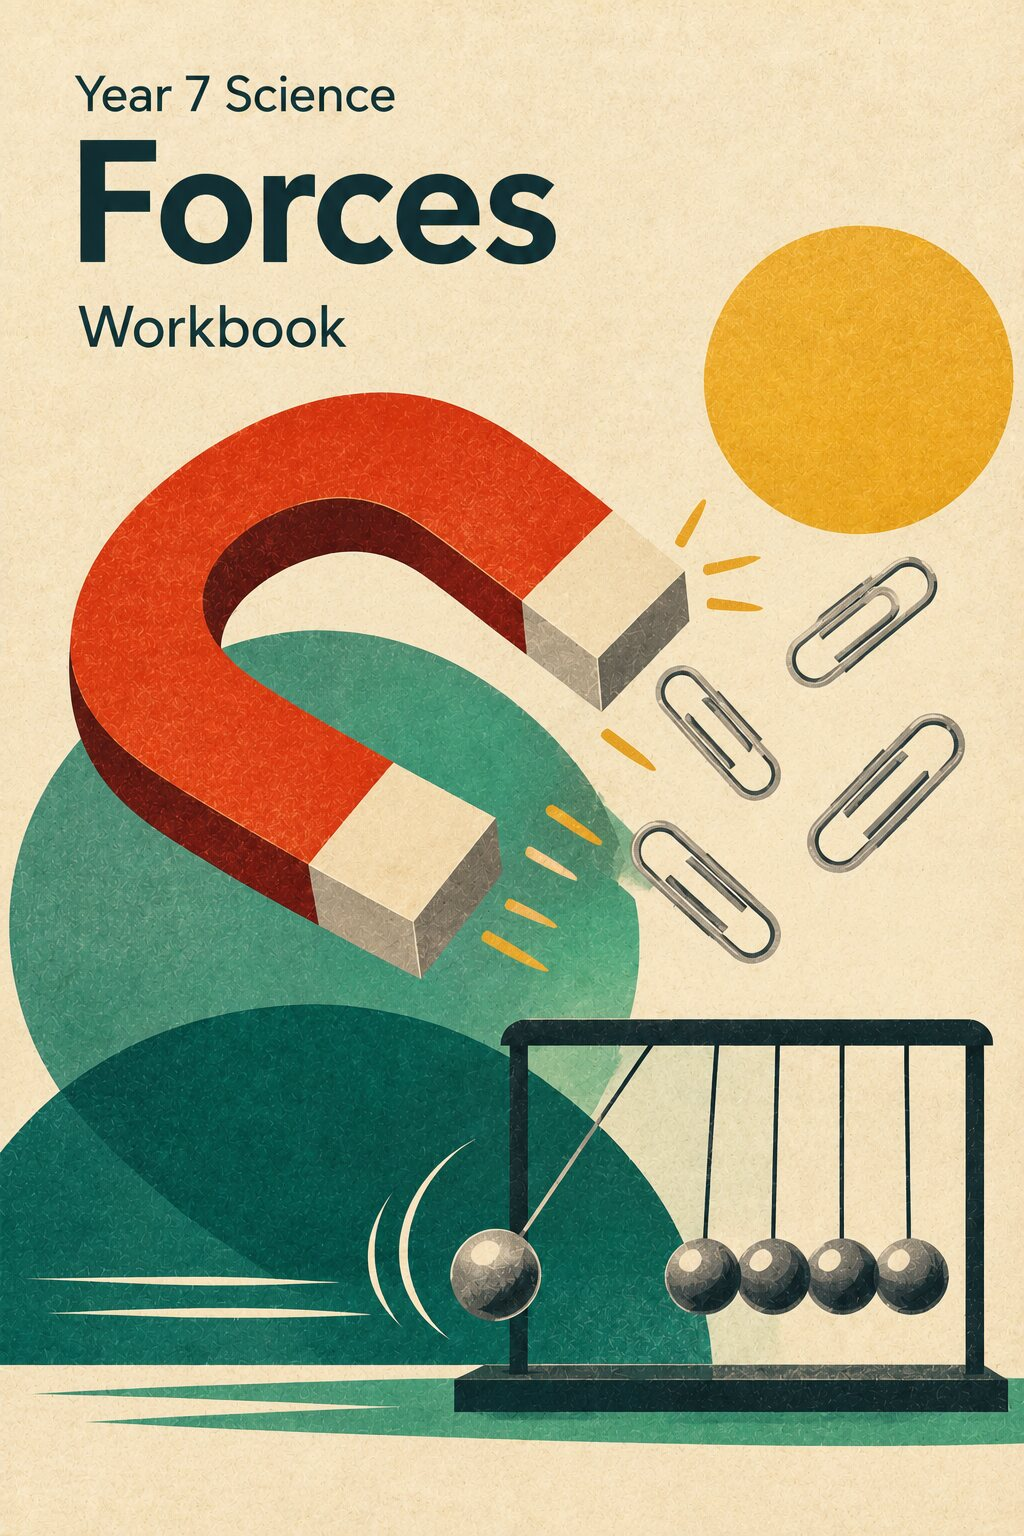
\includegraphics[width=\paperwidth]{../../../covers/forces.jpg}};
  \node[anchor=north east, fill=white, draw=Ink, line width=0.6pt, rounded corners=1.2mm,
        inner xsep=2mm, inner ysep=1.8mm, text width=30mm, font=\headingfont\footnotesize]
    at ([xshift=-4mm, yshift=-4mm]current page.north east)
    {\textbf{Name}\par\vspace{4mm}\hrule\vspace{2mm}\textbf{Class}\par\vspace{4mm}\hrule};
  \node[anchor=south east, fill=white, draw=Ink, line width=0.6pt, rounded corners=1.2mm,
        inner xsep=2.6mm, inner ysep=2mm, font=\headingfont\bfseries, align=right]
    at ([xshift=-4mm, yshift=6mm]current page.south east)
    {Lesson Booklet 1\\[-1pt]{\normalfont\headingfont\scriptsize Lessons 1--4}};
\end{tikzpicture}
\mbox{}
\clearpage

% ---- Inside cover ---------------------------------------------------------
\thispagestyle{plain}
{\headingfont\bfseries\fontsize{22}{26}\selectfont Forces and Motion}\par\vspace{1mm}
{\headingfont\large Lesson Booklet 1 \textbullet\ Lessons 1--4 \textbullet\ Year 7}\par\vspace{1mm}
{\small\itshape VC 2.0: VC2S8U13 \textbullet\ VC2S8U14 \textbullet\ VC2S8U15 \textbullet\ VC2S8I01--I08}\par\vspace{4mm}
\textbf{Teacher}\ \hrulefill\par

\begin{countrybox}{Acknowledgement of Country}
This booklet was created on the unceded Country of the Wurundjeri Woi-wurrung people of the Kulin Nation. We acknowledge Elders past, present and emerging.
\end{countrybox}

\begin{infobox}{How this booklet works}
One section for each lesson. Each opens with its key vocabulary, then:\par\smallskip
\renewcommand{\arraystretch}{1.25}
\begin{tabular}{@{}p{24mm}p{70mm}@{}}
\textbf{Part A} & a reading with comprehension questions \\
\textbf{Part B} & the ideas, worked through \\
\textbf{Part C} & practice on your own \\
\textbf{Part D} & above level: Year 8 extension \\
\end{tabular}

\smallskip
\begin{tabular}{@{}p{24mm}p{70mm}@{}}
\textbf{I do} \tagicon{\icodots{1}} & your teacher works an example (solid frame) \\
\textbf{We do} \tagicon{\icodots{2}} & you try one together (dashed frame) \\
\textbf{Reading} \tagicon{\icoread} & a passage to read (thin frame) \\
\textbf{Above level} \tagicon{\icoup} & extension (double frame) \\
\end{tabular}

\smallskip
Three lesson books. The five experiments are in the \textbf{Experiment Booklet}; the trebuchet investigation has its own booklet.
\end{infobox}

\clearpage
\markboth{Contents}{Contents}
{\headingfont\bfseries\LARGE Contents}\par\vspace{1mm}\noindent\rule{\linewidth}{0.6pt}\par\vspace{2mm}
\renewcommand{\arraystretch}{1.12}
\begin{tabular}{|C{1.1cm}|L{6.0cm}|C{2.4cm}|}
  \hline\thead{Lesson} & \thead{Title} & \thead{Page} \\ \hline
  1 & \hyperlink{lesson.1.1}{What is a Force?} & \hyperlink{lesson.1.1}{p.\ \pageref{sec:1}} \\ \hline
  2 & \hyperlink{lesson.2.1}{Force Diagrams and Net Force} & \hyperlink{lesson.2.1}{p.\ \pageref{sec:2}} \\ \hline
  3 & \textit{Experiment 1 --- Everyday Forces} & {\footnotesize Experiment Booklet} \\ \hline
  4 & \hyperlink{lesson.4.1}{Newton's First and Third Laws} & \hyperlink{lesson.4.1}{p.\ \pageref{sec:4}} \\ \hline
  5 & Newton's Second Law: \texorpdfstring{$F = ma$}{F = ma} & Book 2 \\ \hline
  6 & \textit{Experiment 2 --- Friction and Mass} & {\footnotesize Experiment Booklet} \\ \hline
  7 & Energy and Transformation & Book 2 \\ \hline
  8 & \textit{Experiment 3 --- Bounce Efficiency} & {\footnotesize Experiment Booklet} \\ \hline
  9 & Simple Machines and Levers & Book 2 \\ \hline
  10 & \textit{Experiment 4 --- Lever Mechanical Advantage} & {\footnotesize Experiment Booklet} \\ \hline
  11 & Levers Extension (Optional) & Book 3 \\ \hline
  12 & Projectile Motion & Book 3 \\ \hline
  13 & \textit{Experiment 5 --- Measuring $g$} & {\footnotesize Experiment Booklet} \\ \hline
  14 & Optimising Range (Optional) & Book 3 \\ \hline
  15 & \textit{Trebuchet investigation: planning} & {\footnotesize Trebuchet booklet} \\ \hline
  16 & \textit{Trebuchet investigation: launches} & {\footnotesize Trebuchet booklet} \\ \hline
  17 & \textit{Trebuchet investigation: analysis and conclusion} & {\footnotesize Trebuchet booklet} \\ \hline
  --- & \hyperlink{glossary}{Glossary} & \hyperlink{glossary}{\pageref{sec:glossary}} \\ \hline
\end{tabular}
\renewcommand{\arraystretch}{1}
\clearpage
\setcounter{section}{0}\renewcommand{\lessonart}{1}
% ══════════════════════════════════════════════════════════════════════════════
%  LESSON 1 — WHAT IS A FORCE?                                    (Week 1 · P1)
% ══════════════════════════════════════════════════════════════════════════════
\sectiondiv{What is a Force?}{Pushes and pulls \textbullet{} Measuring force \textbullet{} Mass and weight \textbullet{} Contact and non-contact forces}\label{sec:1}
\lessoncodes{VC2S8U14 \textbullet{} VC2S8I04}

\vocabhead
\begin{ctab}
\begin{tabular}{|SW{2.91cm}|W{8.05cm}|}
  \hd & \thead{Word} & \thead{Definition (copy from the slide)} \\ \hline
  & \scaf{\textbf{Force}\label{voc:force}} & \scaf{A push or a pull on an object.} \\ \hline
  & \textbf{Newton (N)}\label{voc:newton-n} & \cell{1.v2} \\ \hline
  & \textbf{Spring scale}\label{voc:spring-scale} & \cell{1.v3} \\ \hline
  & \textbf{Mass}\label{voc:mass} & \cell{1.v4} \\ \hline
  & \textbf{Weight}\label{voc:weight} & \cell{1.v5} \\ \hline
  & \textbf{Non-contact force}\label{voc:non-contact-force} & \cell{1.v6} \\ \hline
\end{tabular}
\end{ctab}

% ─── PART A ───────────────────────────────────────────────────────────────────
\lessonpart{A}{Reading and comprehension}{Teal}\label{read:1}

\begin{readingbox}{Reading --- The Forces You Cannot See}
Right now, while you sit perfectly still, you are being pushed and pulled from several directions at once. Gravity is pulling every part of your body downwards towards the centre of the Earth. At the same time, the chair beneath you is pushing upwards on you with exactly the same strength. Because these two forces are equal and opposite, you stay put. If the chair suddenly vanished, the pushing force would disappear, gravity would win, and you would fall.

People often think that astronauts on the International Space Station float because there is no gravity in space. This is not true. At the height the Space Station orbits, Earth's gravity is still about 90\% as strong as it is on the ground. Astronauts float because they --- and the whole Space Station --- are falling around the Earth at enormous speed, and they fall together. Everything inside falls at the same rate, so nothing presses against anything else. The astronauts do not feel the push of a floor, so they seem weightless.

Forces are invisible, so scientists need a way to record them. The solution is simple but powerful: draw each force as an arrow. The direction of the arrow shows which way the force acts, and the length of the arrow shows how strong it is. A picture full of invisible pushes and pulls becomes something you can measure, compare and calculate with.
\end{readingbox}

\rcreset
\rcqk{1.c1}{According to the passage, name the two forces acting on you while you sit still, and state the direction of each.}{1.6cm}
\rcqk{1.c2}{The passage says that if the chair vanished, ``gravity would win''. Explain what this means, using the idea of two forces that are no longer equal.}{1.8cm}
\rcqk{1.c3}{Explain why astronauts on the Space Station appear to float, even though gravity is still acting on them.}{2.2cm}
\rcqk{1.c4}{Does an astronaut on the Space Station still have weight? Use a number from the passage to support your answer.}{1.6cm}
\clearpage
\rcqk{1.c5}{The passage says drawing forces as arrows is ``simple but powerful''. What two pieces of information does a force arrow give you?}{1.6cm}
\rcqk{1.c6}{Which three-word phrase in the first paragraph describes two forces that are the same size but act in opposite directions?}{1.4cm}
\rcqk{1.c7}{Forces are invisible. Describe one way you could tell that a force is acting on an object, even though you cannot see the force itself.}{1.8cm}
\rcqk{1.c8}{Imagine the Space Station suddenly stopped moving around the Earth. Using the passage, predict what would happen to the station and the astronauts inside, and explain why.}{2.2cm}

% ─── PART B ───────────────────────────────────────────────────────────────────
\lessonpart{B}{Theory and examples}{Blue}\label{theory:1}

\subsection{Every Force is a Push or a Pull}\label{sub:1.1}

This is the whole idea, and it really is that simple. Whenever one object affects another --- by touching it, or from a distance --- it does so by \textbf{pushing} it or \textbf{pulling} it. There is no third option.

\begin{skillbox}{Think about it}
A magnet \emph{pulls} a paperclip. A hand \emph{pushes} a door. The Earth \emph{pulls} you downwards. A rope \emph{pulls} a sledge. The ground \emph{pushes} up on your feet.
\end{skillbox}

\subsection{What Forces Can Do}\label{sub:1.2}

A force can only change an object in a small number of ways. Learn these five and you can describe almost any situation in this unit.

\vspace{4pt}
\begin{ctab}
\begin{tabular}{|C{0.57cm}|L{3.99cm}|L{5.98cm}|}
  \thead{\#} & \thead{A force can\ldots} & \thead{Example} \\ \hline
  \talt 1 & Make a still object start moving   & A kicked football leaves the ground \\ \hline
        2 & Make a moving object stop          & Brakes bring a bicycle to a halt \\ \hline
  \talt 3 & Make an object speed up or slow down & Pedalling harder makes you accelerate \\ \hline
        4 & Change the direction of motion     & A tennis racquet sends the ball back \\ \hline
  \talt 5 & Change the shape of an object      & Squashing a drink can \\ \hline
\end{tabular}
\end{ctab}

\subsection{Measuring Force: The Newton}\label{sub:1.3}

Force is measured in \textbf{newtons}, written \textbf{N}. The unit is named after Sir Isaac Newton, whose laws of motion you will meet in Lesson~4.

\begin{infobox}{Getting a feel for a newton}
\textbf{1 N} is roughly the force you feel holding a small apple (about 100 g) against gravity.\\
\textbf{10 N} is about the weight of a 1 kg bag of sugar.\\
\textbf{500 N} is roughly the weight of an average adult.
\end{infobox}

We measure force with a \textbf{spring scale} (also called a \emph{newton meter}). Inside is a spring: the harder you pull, the further it stretches, and a pointer moves down a scale marked in newtons.

\vspace{4pt}
\diagSpringScales
\figcap[fig:spring-scale]{Reading a spring scale. Always read at eye level, and check the size of each small division first.}

\begin{skillbox}{How to read a spring scale correctly}
\begin{enumerate}[itemsep=1pt, leftmargin=1.4em, topsep=1pt]
  \item Check the \textbf{largest} number on the scale --- this is the maximum it can measure.
  \item Work out what \textbf{one small division} is worth. If there are 10 small gaps between 0 and 5 N, each is 0.5 N.
  \item Hold the scale still and read at \textbf{eye level} to avoid parallax error.
  \item Read the value where the \textbf{pointer} sits, and always write the \textbf{unit (N)}.
\end{enumerate}
\end{skillbox}

\begin{workedex}{Reading a spring scale}
A spring scale is marked from 0 to 10\,N, with \textbf{20} small divisions between 0 and 10. The pointer sits on the \textbf{7th} small division. What is the reading?

\medskip
\textbf{Step 1 --- one division:}\quad $10 \div 20 = 0.5$\,N per division

\textbf{Step 2 --- the reading:}\quad $7 \times 0.5 = \mathbf{3.5\ \text{N}}$
\end{workedex}

\begin{wedo}{Reading a spring scale}
A spring scale is marked from 0 to 5\,N, with \textbf{20} small divisions between 0 and 5. The pointer sits on the \textbf{9th} small division. What is the reading?
\par\smallskip\noindent
\begin{minipage}[c]{0.3\linewidth}\diagSpringScaleWeDo\end{minipage}\hfill
\begin{minipage}[c]{0.66\linewidth}\wbox{1.wd1}{4.6cm}\end{minipage}
\end{wedo}

\subsection{Mass and Weight Are Not the Same Thing}\label{sub:1.4}

In everyday speech we use these words as if they mean the same thing. In science they are quite different, and mixing them up causes a lot of lost marks.

\vspace{4pt}
\begin{ctab}
\begin{tabular}{|L{2.22cm}|L{4.16cm}|L{4.16cm}|}
  \thead{} & \thead{Mass} & \thead{Weight} \\ \hline
  \talt What it is   & The amount of matter in an object & The \emph{force} of gravity pulling on that mass \\ \hline
        Unit         & kilograms (kg)                    & newtons (N) \\ \hline
  \talt Measured with& A balance                         & A spring scale \\ \hline
        Changes?     & Same everywhere in the universe   & Changes with the strength of gravity \\ \hline
\end{tabular}
\end{ctab}

\begin{infobox}{The link between them}
\[ \text{Weight} = \text{mass} \times \text{gravitational field strength} \qquad\Rightarrow\qquad \boxed{W = mg} \]
On Earth, $g = 9.8$\,N/kg. On the Moon, $g = 1.6$\,N/kg.
\end{infobox}

\begin{workedex}{Mass and weight}
A student has a mass of 50\,kg. Find their weight on Earth, and on the Moon.

\medskip
\textbf{On Earth:}\quad $W = mg = 50 \times 9.8 = \mathbf{490\ \text{N}}$

\textbf{On the Moon:}\quad $W = mg = 50 \times 1.6 = \mathbf{80\ \text{N}}$

\medskip
Their \emph{mass} is 50\,kg in both places --- only the \emph{weight} changes.
\end{workedex}

\begin{wedo}{Mass and weight}
A robot has a mass of 20\,kg. Use $g = 9.8$\,N/kg on Earth and $g = 1.6$\,N/kg on the Moon.
\pt{a}Find its weight on Earth.
\wbox{1.wd2a}{1.8cm}
\pt{b}Find its weight on the Moon.
\wbox{1.wd2b}{1.8cm}
\pt{c}Has its mass changed? Explain.
\abox{1.wd2c}{1.6cm}
\end{wedo}

\subsection{Contact and Non-contact Forces}\label{sub:1.5}

Forces fall into two groups. \textbf{Contact forces} only act when two objects touch. \textbf{Non-contact forces} act across a gap --- the objects do not need to touch at all.

\vspace{4pt}
\diagForceTypes
\figcap{Contact and non-contact forces}

\needspace{14\baselineskip}
\begin{workedex}{Classifying forces}
A fridge magnet holds a shopping list on the fridge door without sliding down. Name two forces acting on the magnet and classify each one.

\medskip
\textbf{Weight} pulls the magnet down --- gravity acts across a gap, so it is a \textbf{non-contact} force.

\textbf{Friction} between the magnet and the door stops it sliding --- the surfaces must touch, so it is a \textbf{contact} force.

\medskip
\textit{(The magnetic pull towards the door is also non-contact --- it is what presses the magnet on hard enough for friction to hold it.)}
\end{workedex}

\begin{wedo}{Classifying forces}
A book is pushed across a desk. After you let go, it slides and slows down. Name two forces acting on the book while it slides, and say whether each one is a contact or a non-contact force.
\abox{1.wd3}{4.0cm}
\end{wedo}

% ─── PART C ───────────────────────────────────────────────────────────────────
\lessonpart{C}{Practice}{Amber}\label{prac:1}

Work through every task. Show your working for calculations, and always include the unit.

\needspace{10\baselineskip}
\task For each everyday action, decide whether the force is a push or a pull. Write \textbf{PUSH} or \textbf{PULL} in the box.

\vspace{4pt}
\begin{ctab}
\begin{tabular}{|SW{3.51cm}|Z{1.55cm}|W{3.51cm}|Z{1.55cm}|}
  \hd & \thead{Action} & \thead{Push or pull?} & \thead{Action} & \thead{Push or pull?} \\ \hline
  & Kicking a football      & \scaf{PUSH} & Opening a drawer       & \scaf{PULL} \\ \hline
  & A crane lifting a girder & \cell{1.t1-r2c2} & Squeezing a stress ball & \cell{1.t1-r2c4} \\ \hline
  & A dog straining on a lead & \cell{1.t1-r3c2} & Wind on a sail       & \cell{1.t1-r3c4} \\ \hline
\end{tabular}
\end{ctab}

\needspace{10\baselineskip}
\task For each event below, write the \textbf{number} of the effect the force is having. Some events have more than one.

\vspace{2pt}
\begin{ctab}
\begin{tabular}{|C{1.88cm}|C{1.88cm}|C{2.17cm}|C{1.88cm}|C{1.88cm}|}
  \thead{1} & \thead{2} & \thead{3} & \thead{4} & \thead{5} \\ \hline
  starts it moving & stops it & speeds it up or slows it down & changes its direction & changes its shape \\ \hline
\end{tabular}
\end{ctab}

\vspace{3pt}
\begin{ctab}
\begin{tabular}{|SW{3.78cm}|Z{1.28cm}|W{3.78cm}|Z{1.28cm}|}
  \hd & \thead{Event} & \thead{Effect (1--5)} & \thead{Event} & \thead{Effect (1--5)} \\ \hline
  & A goalkeeper catches a ball  & \scaf{2} & Stretching a rubber band & \scaf{5} \\ \hline
  & A car turns a corner at steady speed & \cell{1.t2-r2c2} & A rocket lifts off & \cell{1.t2-r2c4} \\ \hline
\end{tabular}
\end{ctab}

\needspace{14\baselineskip}
\task Think of three forces you used this morning. For each one, describe the action, write \textbf{PUSH} or \textbf{PULL}, and give the number of the effect it had: \textbf{1} starts it moving, \textbf{2} stops it, \textbf{3} speeds it up or slows it down, \textbf{4} changes its direction, \textbf{5} changes its shape.

\vspace{3pt}
\begin{ctab}
\begin{tabular}{|SW{6.32cm}|Z{2.11cm}|Z{2.11cm}|}
  \hd & \thead{Action} & \thead{Push or pull?} & \thead{Effect (1--5)} \\ \hline
  & \scaf{Opening the fridge door} & \scaf{PULL} & \scaf{1} \\ \hline
  & \cell{1.t3-r2c1} & \cell{1.t3-r2c2} & \cell{1.t3-r2c3} \\ \hline
  & \cell{1.t3-r3c1} & \cell{1.t3-r3c2} & \cell{1.t3-r3c3} \\ \hline
  & \cell{1.t3-r4c1} & \cell{1.t3-r4c2} & \cell{1.t3-r4c3} \\ \hline
\end{tabular}
\end{ctab}

\needspace{24\baselineskip}
\task Write the reading shown on each of the three spring scales below. Check what one small division is worth on each scale first.

\diagSpringScales

\vspace{3pt}
\begin{ctab}
\begin{tabular}{|SZ{3.51cm}|Z{3.51cm}|Z{3.51cm}|}
  \hd & \thead{Scale A} & \thead{Scale B} & \thead{Scale C} \\ \hline
  & \cell{1.t4-r1c1} & \cell{1.t4-r1c2} & \cell{1.t4-r1c3} \\ \hline
\end{tabular}
\end{ctab}

\needspace{10\baselineskip}
\task Complete the table. Use $g = 9.8$\,N/kg on Earth and $g = 1.6$\,N/kg on the Moon.

\vspace{3pt}
\begin{ctab}
\begin{tabular}{|SW{3.19cm}|Z{1.94cm}|Z{2.50cm}|Z{2.50cm}|}
  \hd & \thead{Object} & \thead{Mass (kg)} & \thead{Weight on Earth (N)} & \thead{Weight on Moon (N)} \\ \hline
  & Bag of sugar & 1   & \scaf{$1 \times 9.8 = 9.8$} & \scaf{$1 \times 1.6 = 1.6$} \\ \hline
  & Bicycle      & 12  & \cell{1.t5-r2c3} & \cell{1.t5-r2c4} \\ \hline
  & Small car    & 900 & \cell{1.t5-r3c3} & \cell{1.t5-r3c4} \\ \hline
\end{tabular}
\end{ctab}

\taskpair{A bag of flour has a mass of 2\,kg. Find its weight on Earth. Use $g = 9.8$\,N/kg.}{\wbox{1.t6}{2.2cm}}
         {Which has the greater weight on Earth: a 5\,kg dog, or a box that weighs 50\,N? Show your working.}{\wbox{1.t7}{2.2cm}}

\needspace{10\baselineskip}
\task Complete the table. For each force, write whether it is a contact or non-contact force, and give a real-world example.

\vspace{4pt}
\begin{ctab}
\begin{tabular}{|SW{2.45cm}|Z{2.45cm}|W{5.63cm}|}
  \hd & \thead{Force} & \thead{Contact / Non-contact} & \thead{Real-world example} \\ \hline
  & Gravity        & \scaf{Non-contact} & \scaf{An apple falling from a tree} \\ \hline
  & Friction       & \cell{1.t8-r2c2} & \cell{1.t8-r2c3} \\ \hline
  & Magnetic force & \cell{1.t8-r3c2} & \cell{1.t8-r3c3} \\ \hline
  & Normal force   & \cell{1.t8-r4c2} & \cell{1.t8-r4c3} \\ \hline
  & Air resistance & \cell{1.t8-r5c2} & \cell{1.t8-r5c3} \\ \hline
  & Tension        & \cell{1.t8-r6c2} & \cell{1.t8-r6c3} \\ \hline
\end{tabular}
\end{ctab}


\needspace{10\baselineskip}
\task A spring scale is marked from 0 to 20\,N, with \textbf{40} small divisions. The pointer sits on the \textbf{13th} small division. What is the reading? Show both steps.
\wbox{1.t9}{2.2cm}

\taskpair{A cat has a mass of 4\,kg. Find its weight on Earth.}{\wbox{1.t10}{2.2cm}}
         {The same cat travels to the Moon. Find its weight there. Has its mass changed?}{\wbox{1.t11}{2.2cm}}

\needspace{10\baselineskip}
\task A balloon rubbed on your hair sticks to a wall. Name the force holding it there, and say whether it is a contact or non-contact force.
\abox{1.t12}{2.0cm}

% ─── PART D ───────────────────────────────────────────────────────────────────
\lessonpart{D}{Above level}{Violet}\label{ext:1}

\begin{yr8box}
These questions go beyond the Year 7 standard. They ask you to combine ideas, use a formula, or judge someone else's reasoning.

\medskip
\needspace{10\baselineskip}
\exttask An astronaut has a mass of 75\,kg.
\pt{a}Find her weight on Earth.
\wbox{1.x13a}{2.0cm}
\pt{b}Find her weight on the Moon.
\wbox{1.x13b}{2.0cm}
\pt{c}Explain why she can jump much higher on the Moon, even though her mass has not changed.
\abox{1.x13c}{2.0cm}


\needspace{10\baselineskip}
\exttask A suitcase has a weight of 196\,N on Earth.
\pt{a}Find its mass.
\wbox{1.x14a}{2.0cm}
\pt{b}Find its weight on the Moon.
\wbox{1.x14b}{2.0cm}

\needspace{10\baselineskip}
\exttask A bathroom scale really measures \emph{force}, but it is labelled in kilograms. A 60\,kg student reads 60\,kg on it on Earth. Predict what the same scale would read on the Moon, and explain why the scale is not really measuring mass.
\abox{1.x15}{3.0cm}

\needspace{10\baselineskip}
\exttask On Mars, $g = 3.7$\,N/kg. A 10\,kg backpack is carried on Earth ($g = 9.8$\,N/kg), on the Moon ($g = 1.6$\,N/kg) and on Mars.
\pt{a}Calculate the backpack's weight in each place.
\wbox{1.x16a}{2.0cm}
\pt{b}Rank the three places from easiest to hardest to carry the backpack, and explain your ranking.
\abox{1.x16b}{2.0cm}

\needspace{10\baselineskip}
\exttask A rock hangs from a spring scale on Earth, and the scale reads 4.9\,N. Use $g = 9.8$\,N/kg on Earth and $g = 1.6$\,N/kg on the Moon.
\pt{a}Find the mass of the rock.
\wbox{1.x17a}{2.0cm}
\pt{b}Find what the same spring scale would read if the rock were hung from it on the Moon.
\wbox{1.x17b}{2.0cm}

\needspace{10\baselineskip}
\exttask A \emph{balance} compares an object with known masses. A \emph{spring scale} measures the pull of gravity on the object. Explain why a balance gives the same result on the Moon as on Earth, but a spring scale does not.
\abox{1.x18}{3.2cm}

\needspace{10\baselineskip}
\exttask Magnets can push or pull without touching. Describe a quick test you could do with a magnet, a paperclip and a sheet of paper to show that magnetic force acts \emph{through} the paper. Say what you would do and what you would expect to see.
\abox{1.x19}{3.4cm}

\end{yr8box}
\newpage
\setcounter{section}{1}\renewcommand{\lessonart}{2}
% ══════════════════════════════════════════════════════════════════════════════
%  LESSON 2 — FORCE DIAGRAMS AND NET FORCE                        (Week 1 · P2)
% ══════════════════════════════════════════════════════════════════════════════
\sectiondiv{Force Diagrams and Net Force}{Naming forces \textbullet{} Force arrows \textbullet{} Free body diagrams \textbullet{} Balanced and unbalanced forces}\label{sec:2}
\lessoncodes{VC2S8U14 \textbullet{} VC2S8I04}

\vocabhead
\begin{ctab}
\begin{tabular}{|SW{2.91cm}|W{8.05cm}|}
  \hd & \thead{Word} & \thead{Definition (copy from the slide)} \\ \hline
  & \scaf{\textbf{Free body diagram}\label{voc:free-body-diagram}} & \scaf{A drawing of one object with an arrow for every force acting on it.} \\ \hline
  & \textbf{Normal force}\label{voc:normal-force} & \cell{2.v2} \\ \hline
  & \textbf{Friction}\label{voc:friction} & \cell{2.v3} \\ \hline
  & \textbf{Air resistance}\label{voc:air-resistance} & \cell{2.v4} \\ \hline
  & \textbf{Net force}\label{voc:net-force} & \cell{2.v5} \\ \hline
  & \textbf{Unbalanced forces}\label{voc:unbalanced-forces} & \cell{2.v6} \\ \hline
\end{tabular}
\end{ctab}

% ─── PART A ───────────────────────────────────────────────────────────────────
\lessonpart{A}{Reading and comprehension}{Teal}\label{read:2}

\begin{readingbox}{Reading --- Winning a Tug-of-War}
In a tug-of-war, two teams pull on the same rope in opposite directions. While the rope stays still, the two pulls are exactly the same size. They are \emph{balanced}, so the net force on the rope is zero --- the rope does not move, even though both teams are pulling as hard as they can.

The moment one team pulls even a little harder, the forces become \emph{unbalanced}. There is now a net force towards the stronger team, and the rope starts to move their way. The bigger the difference between the two pulls, the faster the rope speeds up.

So how does a team pull harder? Strength helps, but the real secret is under their feet. To pull on the rope, each person pushes backwards against the ground with their shoes. Friction between the shoes and the ground stops them from sliding forwards. A team with good grip --- rough soles, a dry surface, bodies low and leaning back --- can pull harder before their feet slip. A team on a slippery surface will be dragged across, no matter how strong they are.

Coaches explain this with force arrows. They draw the rope, the two pulls and the friction on the feet, each as an arrow whose length shows its size. One look at the arrows shows which team is going to win.
\end{readingbox}

\rcreset
\rcqk{2.c1}{While the rope is not moving, what can you say about the two teams' pulls? Use the word \emph{balanced}.}{1.6cm}
\rcqk{2.c2}{What happens to the rope when one team pulls harder? Explain why, using the words \emph{net force}.}{1.8cm}
\rcqk{2.c3}{According to the passage, why does a team on a slippery surface lose, however strong they are?}{1.8cm}
\rcqk{2.c4}{List two things from the passage that give a team better grip.}{1.4cm}
\rcqk{2.c5}{How can a coach tell which team will win just by looking at the force arrows?}{1.6cm}
\rcqk{2.c6}{Explain why each person needs friction under their shoes in order to pull on the rope.}{1.8cm}
\rcqk{2.c7}{A team plays in socks on a polished wooden floor. Use the passage to predict what will happen to them, and explain why.}{1.8cm}
\rcqk{2.c8}{In your own words, explain the difference between balanced and unbalanced forces. Give an example of each from the passage.}{2.2cm}

% ─── PART B ───────────────────────────────────────────────────────────────────
\lessonpart{B}{Theory and examples}{Blue}\label{theory:2}

\subsection{Naming the Forces}\label{sub:2.1}

Before you can draw a force diagram, you need the right names. These are the forces you will use again and again in this unit.

\vspace{4pt}
\begin{ctab}
\begin{tabular}{|L{2.36cm}|L{4.44cm}|L{3.74cm}|}
  \thead{Force} & \thead{What causes it} & \thead{Which way it acts} \\ \hline
  \talt Weight ($W$)        & Gravity pulling on mass              & Always straight down \\ \hline
        Normal force ($N$)  & A surface pushing back on an object  & Perpendicular to the surface \\ \hline
  \talt Friction ($f$)      & Two surfaces rubbing together        & Opposite to the motion \\ \hline
        Air resistance      & Air pushing against a moving object  & Opposite to the motion \\ \hline
  \talt Tension ($T$)       & A rope, string or cable pulling      & Along the rope, away from the object \\ \hline
        Applied force       & A person or machine pushing/pulling  & Whichever way it is applied \\ \hline
\end{tabular}
\end{ctab}

\subsection{Drawing Force Arrows --- The Three Rules}\label{sub:2.2}

\begin{skillbox}{The three rules for every force arrow}
\begin{enumerate}[itemsep=2pt, leftmargin=1.4em, topsep=1pt]
  \item \textbf{Start the arrow on the object.} The tail sits on the object the force acts on.
  \item \textbf{Point the arrowhead the way the force acts.} Down for weight, up for the normal force, and so on.
  \item \textbf{Make the length match the size.} A 20\,N force is drawn twice as long as a 10\,N force. \emph{Always}.
\end{enumerate}
\end{skillbox}

Rule 3 is the one students most often forget --- and it matters, because the picture should tell you the answer at a glance. If two arrows are the same length, the forces are balanced. If one is longer, that is the direction the object accelerates.

\vspace{4pt}
\diagArrowScale
\figcap{Using a scale for force arrows. Here 1\,cm represents 5\,N, so a 15\,N force is drawn 3\,cm long.}

\begin{workedex}{Drawing arrows to scale}
Using a scale of 1\,cm = 5\,N, how long should the arrow be for a 25\,N push?

\medskip
\textbf{Length} $=$ force $\div$ scale $= 25 \div 5 = \mathbf{5\ \text{cm}}$
\end{workedex}

\begin{wedo}{Drawing arrows to scale}
Using a scale of 1\,cm = 10\,N:
\pt{a}Work out how long the arrow should be for a 40\,N pull.
\wbox{2.wd1a}{1.8cm}
\pt{b}Draw the arrow, starting on the dot, pointing to the right. Label it with its size.
\drawk{2.wd1b}{2.4cm}{\vspace*{0.6cm}\tikz{\fill[Ink] (0,0) circle (2.5pt);}}
\end{wedo}

\subsection{Free Body Diagrams}\label{sub:2.3}

A \textbf{free body diagram (FBD)} shows \emph{all} the forces acting on \emph{one} object, each drawn as a labelled arrow using the three rules. The object is drawn as a simple box or dot --- nothing else from the picture is included.

\diagFBD
\figcap[fig:fbd]{Balanced forces (left) and unbalanced forces (right)}

\begin{workedex}{Drawing a free body diagram}
A book with a weight of 10\,N rests on a table. Draw its free body diagram.

\medskip
\textbf{Step 1 --- find every force.} Gravity pulls the book down (\emph{weight}). The table pushes up on it (\emph{normal force}).

\textbf{Step 2 --- size each force.} The book is not moving up or down, so the table pushes up exactly as hard as gravity pulls down: both are 10\,N.

\textbf{Step 3 --- draw.} A box for the book, a 10\,N arrow down labelled $W$, and an arrow of the \emph{same length} up labelled $N$ --- as in the left of Figure~\ref{fig:fbd}.
\end{workedex}

\begin{wedo}{Drawing a free body diagram}
A box is dragged across the floor by a rope at a \textbf{steady speed}. The rope pulls it with 30\,N. The box has a weight of 50\,N. Draw its free body diagram. Label all four forces with their names and sizes, and make the arrow lengths match.
\drawk{2.wd2}{5.0cm}{}
\end{wedo}

\subsection{Balanced and Unbalanced: Net Force}\label{sub:2.4}

When you add up all the forces on an object, the single force left over is called the \textbf{net force} (or resultant force).

\begin{infobox}{Working out the net force}
\textbf{Same direction} $\rightarrow$ \textbf{add} the forces.\\
\textbf{Opposite directions} $\rightarrow$ \textbf{subtract} the smaller from the larger. The net force acts in the direction of the larger force.\\[3pt]
If the net force is \textbf{zero}, the forces are \textbf{balanced} and the motion does not change.\\
If the net force is \textbf{not zero}, the forces are \textbf{unbalanced} and the object speeds up, slows down or changes direction.
\end{infobox}

\begin{workedex}{Finding the net force}
A sledge is pulled forwards with 45\,N. Friction pushes back with 18\,N. Find the net force.

\medskip
Opposite directions, so subtract: \quad $45 - 18 = \mathbf{27\ \text{N forwards}}$

\medskip
The net force is not zero, so the forces are unbalanced and the sledge \textbf{speeds up}.
\end{workedex}

\begin{wedo}{Finding the net force}
A cyclist pedals forwards with a force of 120\,N. Air resistance and friction push back with a total of 75\,N.
\pt{a}Find the size and direction of the net force.
\wbox{2.wd3a}{1.8cm}
\pt{b}Are the forces balanced or unbalanced? Describe what happens to the cyclist's speed.
\abox{2.wd3b}{1.8cm}
\end{wedo}

% ─── PART C ───────────────────────────────────────────────────────────────────
\lessonpart{C}{Practice}{Amber}\label{prac:2}

Work through every task. Show your working for calculations, and always include the unit.

\needspace{10\baselineskip}
\task Using a scale of \textbf{1\,cm = 2\,N}, how long should the arrow be for each force?
\pt{a}6\,N
\wbox{2.t1a}{2.0cm}
\pt{b}10\,N
\wbox{2.t1b}{2.0cm}
\pt{c}3\,N
\wbox{2.t1c}{2.0cm}

\taskpair{Using a scale of 1\,cm = 10\,N, how long should the arrow be for a 45\,N pull?}{\wbox{2.t2}{2.0cm}}
         {An arrow is 3.5\,cm long. The scale is 1\,cm = 20\,N. What force does it show?}{\wbox{2.t3}{2.0cm}}

\needspace{14\baselineskip}
\task A box is pulled right with 30\,N and friction resists with 10\,N. Using a scale of \textbf{1\,cm = 10\,N}, draw both arrows on the box below. Label each with its name and size.

\vspace{3pt}
\drawk{2.t4}{4.2cm}{}

\needspace{24\baselineskip}
\task[a] The diagrams below show the forces on a book resting on a table (left) and on a box being pushed along the floor (right).

\diagFBD
Why is the book not speeding up or slowing down? Use the words \textit{net force} in your answer.
\abox{2.t5a}{2.2cm}

\taskpart{b} The box is pushed right with 20\,N, and friction pushes left with 5\,N. Calculate the net force on the box and state which way it speeds up.
\wbox{2.t5b}{2.2cm}

\needspace{16\baselineskip}
\taskpart{c} Draw a free body diagram for a skydiver falling at a steady speed (terminal velocity). Label each force with its name and show their comparative sizes.

\vspace{3pt}
\drawk{2.t5c}{4.6cm}{
\textit{\color{MidGrey}Draw your force diagram here.}
}

\needspace{14\baselineskip}
\task A lamp with a weight of 15\,N hangs still from the ceiling on a cord. Draw its free body diagram, labelling each force with its name and size.

\vspace{3pt}
\drawk{2.t6}{4.2cm}{
\textit{\color{MidGrey}Draw your force diagram here.}
}

\needspace{6\baselineskip}
\textbf{Net force.} For each question, state the size \emph{and} direction of the net force, and whether the forces are balanced or unbalanced.

\taskpair{Two people push a car in the same direction with 250\,N and 310\,N. Find the net force.}{\wbox{2.t7}{2.2cm}}
         {A trolley is pushed right with 40\,N while friction pushes left with 12\,N. Find the net force.}{\wbox{2.t8}{2.2cm}}

\taskpair{A book rests on a table. Its weight is 8\,N. What is the normal force from the table? Explain.}{\abox{2.t9}{2.2cm}}
         {In a tug-of-war, one team pulls left with 900\,N and the other pulls right with 900\,N. Describe the motion of the rope.}{\abox{2.t10}{2.2cm}}

\needspace{10\baselineskip}
\task A rocket engine produces 50\,000\,N of upward thrust. The rocket's weight is 32\,000\,N.
\pt{a}Find the net force.
\wbox{2.t11a}{2.0cm}
\pt{b}State which way the rocket speeds up.
\abox{2.t11b}{2.0cm}
\pt{c}Explain what would happen if the thrust dropped to 32\,000\,N.
\abox{2.t11c}{2.0cm}

\taskpair{A box has three forces on it: 15\,N right, 10\,N right and 30\,N left. Find the size and direction of the net force.}{\wbox{2.t12}{2.4cm}}
         {A skydiver weighs 600\,N. Air resistance on her is 600\,N. Are the forces balanced or unbalanced? Describe her motion.}{\abox{2.t13}{2.4cm}}

\needspace{10\baselineskip}
\task A swimmer moves forward at a steady speed. Her arms provide 120\,N of forward force.
\pt{a}What is the size of the water resistance acting on her?
\abox{2.t14a}{2.0cm}
\pt{b}Explain how you know.
\abox{2.t14b}{2.0cm}

\needspace{10\baselineskip}
\task A parachutist has a weight of 700\,N. Just after the parachute opens, air resistance is 950\,N.
\pt{a}Find the net force and its direction.
\wbox{2.t15a}{2.0cm}
\pt{b}Describe what happens to the parachutist's speed.
\abox{2.t15b}{2.0cm}
\pt{c}Air resistance then falls to 700\,N --- describe the motion now.
\abox{2.t15c}{2.0cm}


% ─── PART D ───────────────────────────────────────────────────────────────────
\needspace{12\baselineskip}
\task In a tug-of-war, Team A pulls the rope left with 550\,N and Team B pulls it right with 620\,N.
\pt{a}Find the size and direction of the net force on the rope.
\wbox{2.t16a}{2.0cm}
\pt{b}Which team is winning? Explain using the words \emph{unbalanced} and \emph{net force}.
\abox{2.t16b}{2.0cm}
\pt{c}Draw both pulls on the rope below as force arrows, using a scale of 1\,cm = 100\,N. Label each arrow with its size.

\vspace{3pt}
\drawk{2.t16c}{4.4cm}{
\vspace*{2.4cm}
\begin{center}\tikz{\draw[line width=2pt, DarkGrey] (0,0) -- (6,0);}\\[2pt]\textit{\small\color{MidGrey}rope}\end{center}
}

\lessonpart{D}{Above level}{Violet}\label{ext:2}

\begin{yr8box}
These questions go beyond the Year 7 standard. They ask you to combine ideas, use a formula, or judge someone else's reasoning.

\medskip
\needspace{10\baselineskip}
\exttask Sam says: \emph{``A hockey puck sliding across ice at a steady speed must have an unbalanced force pushing it forwards.''} Is Sam right? Use a free body diagram and the idea of net force to explain.
\abox{2.x17}{3.4cm}

\needspace{14\baselineskip}
\exttask A skydiver jumps from a plane. Draw a free body diagram for each moment below. Then explain why air resistance grows, and why the skydiver eventually stops speeding up.
\pt{i}just after jumping
\pt{ii}while still speeding up
\pt{iii}at terminal velocity

\vspace{3pt}
\edef\abgrp{\number\numexpr\value{abox}+1\relax}%
\noindent\begin{minipage}[t]{0.31\linewidth}\drawk{2.x18i}{4.2cm}{\textbf{(i)} just after jumping}\end{minipage}\hfill
\begin{minipage}[t]{0.31\linewidth}\drawk{2.x18ii}{4.2cm}{\textbf{(ii)} speeding up}\end{minipage}\hfill
\begin{minipage}[t]{0.31\linewidth}\drawk{2.x18iii}{4.2cm}{\textbf{(iii)} terminal velocity}\end{minipage}\par\gdef\abgrp{0}
\abox{2.x18-why}{2.6cm}

\needspace{10\baselineskip}
\exttask A car has a driving force of 4500\,N and a total resistive force of 1200\,N.
\pt{a}Calculate the net force.
\wbox{2.x19a}{2.0cm}
\pt{b}State which way the car accelerates.
\abox{2.x19b}{2.0cm}
\pt{c}Suggest one way the driver could make the forces balanced.
\abox{2.x19c}{2.0cm}

\needspace{10\baselineskip}
\exttask A 1200\,kg car has a driving force of 4800\,N. Air resistance and friction total 1500\,N.
\pt{a}Find the net force.
\wbox{2.x20a}{2.0cm}
\pt{b}Use $F = ma$ (acceleration = net force $\div$ mass) to find the acceleration.
\wbox{2.x20b}{2.0cm}
\pt{c}The driving force rises to 6000\,N --- find the new acceleration.
\wbox{2.x20c}{2.0cm}
\needspace{16\baselineskip}
\exttask A car drives along a flat road at a steady 60\,km/h. Draw a free body diagram for the car showing four forces: weight, the normal force, the driving force and the total resistive force. Show which pairs of forces are balanced.

\vspace{3pt}
\drawk{2.x21}{4.6cm}{
\textit{\color{MidGrey}Draw your force diagram here.}
}

\needspace{10\baselineskip}
\exttask A 2\,kg ball is falling. Air resistance pushes up on it with 5\,N. Use $W = mg$ with $g = 9.8$\,N/kg.
\pt{a}Find the weight of the ball.
\wbox{2.x22a}{2.0cm}
\pt{b}Find the size and direction of the net force.
\wbox{2.x22b}{2.0cm}
\pt{c}Is the ball speeding up, slowing down or moving at a steady speed? Explain.
\abox{2.x22c}{2.0cm}

\needspace{10\baselineskip}
\exttask A loaded truck and a small car are both travelling at the same speed. Explain, using the idea of net force, why the truck needs a much bigger braking force to stop in the same distance.
\abox{2.x23}{3.0cm}

\end{yr8box}
\newpage
\setcounter{section}{3}\renewcommand{\lessonart}{4}
% ══════════════════════════════════════════════════════════════════════════════
%  LESSON 4 — NEWTON'S FIRST AND THIRD LAWS                       (Week 2 · P1)
% ══════════════════════════════════════════════════════════════════════════════
\sectiondiv{Newton's First and Third Laws}{Inertia \textbullet{} Why moving things keep moving \textbullet{} Action and reaction \textbullet{} Force pairs}\label{sec:4}
\lessoncodes{VC2S8U14 \textbullet{} VC2S10U17 (above level)}

\vocabhead
\begin{ctab}
\begin{tabular}{|SW{2.91cm}|W{8.05cm}|}
  \hd & \thead{Word} & \thead{Definition (copy from the slide)} \\ \hline
  & \scaf{\textbf{Inertia}\label{voc:inertia}} & \scaf{The tendency of an object to keep doing what it is already doing --- staying still or moving at a steady speed.} \\ \hline
  & \textbf{Newton's First Law}\label{voc:newton-s-first-law} & \cell{4.v2} \\ \hline
  & \textbf{Newton's Third Law}\label{voc:newton-s-third-law} & \cell{4.v3} \\ \hline
  & \textbf{Action--reaction pair}\label{voc:action-reaction-pair} & \cell{4.v4} \\ \hline
  & \textbf{Atmosphere}\label{voc:atmosphere} & \cell{4.v5} \\ \hline
\end{tabular}
\end{ctab}

% ─── PART A ───────────────────────────────────────────────────────────────────
\lessonpart{A}{Reading and comprehension}{Teal}\label{read:4}

\begin{readingbox}{Reading --- Why Rockets Work in Empty Space}
\small % one size down so the whole reading fits on the lesson's first page
When rockets were first proposed as a way of reaching space, some newspapers scoffed at the idea. In 1920 an editorial in the \emph{New York Times} argued that a rocket could never work beyond the atmosphere, because out in the vacuum there would be nothing for the exhaust gases to push against. It seemed like common sense. A swimmer pushes against water, a runner pushes against the ground --- so surely a rocket must push against the air?

The reasoning was wrong, and the mistake came from misunderstanding Newton's Third Law. A rocket does not push against the air behind it. It pushes against \emph{its own exhaust}. The engine hurls a huge mass of hot gas backwards, and by the Third Law the gas pushes the rocket forwards with exactly the same force. Nothing outside the rocket is needed at all. In fact rockets work \emph{better} in space, because there is no air resistance slowing them down.

Out in deep space, something even more surprising happens: a spacecraft can switch its engines off and simply keep going. Far from any planet there is no air and almost nothing pushing or pulling on it, so there is almost no unbalanced force to slow it down. The two \emph{Voyager} space probes were launched in 1977. No engine has pushed them forwards for more than thirty years, yet they are still travelling away from the Sun at more than 55\,000 kilometres per hour. Here on Earth, a ball rolled along the ground soon stops --- but only because friction and air resistance act on it. Take those away, and a moving object just keeps moving.

The \emph{New York Times} eventually printed a correction --- in July 1969, the day after Apollo 11 launched for the Moon, and forty-nine years after the original editorial. It noted, briefly, that further investigation had confirmed the work of Newton in the seventeenth century, and regretted the error.
\end{readingbox}

\rcreset
\rcqk{4.c1}{What mistaken reason did the 1920 editorial give for believing rockets could not work in space?}{1.6cm}
\rcqk{4.c2}{Explain, using Newton's Third Law, what a rocket actually pushes against.}{2.0cm}
\rcqk{4.c3}{The passage says rockets work \emph{better} in space. Give the reason, and name the force that is absent.}{1.6cm}
\rcqk{4.c4}{The \emph{Voyager} probes are still moving fast, even though no engine is pushing them. Explain why they have not slowed down.}{2.0cm}
\rcqk{4.c5}{According to the passage, why does a ball rolled along the ground on Earth soon stop?}{1.6cm}
\rcqk{4.c6}{Which phrase in the second paragraph tells you how the push of the gas on the rocket compares with the push of the rocket on the gas?}{1.4cm}
\rcqk{4.c7}{The editorial's reasoning ``seemed like common sense''. Using the two examples in the passage, explain why it seemed right to many people.}{1.8cm}

% ─── PART B ───────────────────────────────────────────────────────────────────
\lessonpart{B}{Theory and examples}{Blue}\label{theory:4}

\subsection{Newton's First Law --- The Law of Inertia}\label{sub:4.1}

In Lesson~2 you learned that when the forces on an object are balanced, its motion does not change. Nearly 340 years ago, Sir Isaac Newton made this the first of his three laws of motion.

\diagNewtonOne
\figcap[fig:newton-one]{Newton's First Law}

\begin{infobox}{First Law}
\textit{``An object at rest stays at rest, and an object in motion stays in motion at constant velocity, unless acted upon by an unbalanced (net) force.''}

\medskip
\textbf{Inertia} is the tendency of an object to resist changes to its motion. Greater mass $=$ greater inertia.
\end{infobox}

The First Law has two halves, and both say the same thing: \emph{without an unbalanced force, nothing about the motion changes.}

\vspace{4pt}
\begin{ctab}
\begin{tabular}{|L{2.53cm}|L{3.65cm}|L{4.36cm}|}
  \thead{If the object is\ldots} & \thead{With no unbalanced force, it\ldots} & \thead{Example} \\ \hline
  \talt At rest & stays at rest & A book on a shelf never starts sliding by itself \\ \hline
        Moving  & keeps moving at the same speed, in the same direction & A space probe coasting with its engines off \\ \hline
\end{tabular}
\end{ctab}

\begin{skillbox}{Think about it --- why do things on Earth seem to stop by themselves?}
For almost 2000 years, people followed the Greek thinker Aristotle, who taught that a moving object needs a force to \emph{keep} it moving. It seems right: a ball rolled along the ground soon stops. Newton showed that the ball stops because \textbf{friction} and \textbf{air resistance} are acting on it. They are unbalanced forces, and they slow it down. With no friction and no air resistance, the ball would roll on forever.
\end{skillbox}

\newpage % Mass and inertia starts its own page
\subsubsection*{Mass and inertia}
The more mass an object has, the more inertia it has --- so the harder it is to change its motion in \emph{any} way.

\vspace{4pt}
\begin{ctab}
\begin{tabular}{|L{3.22cm}|L{3.66cm}|L{3.66cm}|}
  \thead{} & \thead{Empty shopping trolley} & \thead{Full shopping trolley} \\ \hline
  \talt Mass and inertia      & Small & Large \\ \hline
        Getting it moving     & Easy  & Hard \\ \hline
  \talt Stopping it           & Easy  & Hard \\ \hline
        Steering it round a corner & Easy  & Hard \\ \hline
\end{tabular}
\end{ctab}

\begin{workedex}{At rest stays at rest}
A coin sits on a playing card on top of a glass. The card is flicked quickly sideways. Explain why the coin drops into the glass instead of flying off with the card.

\medskip
\textbf{Step 1 --- before the flick.} The coin is at rest. Its weight pulls down and the card pushes up: the forces are balanced.

\textbf{Step 2 --- the flick.} The big force acts on the \emph{card}, not the coin. Only a tiny friction force acts on the coin, for a very short time.

\textbf{Step 3 --- inertia.} The coin's inertia keeps it at rest where it is. With the card gone, nothing pushes up on the coin, so its weight is now \textbf{unbalanced} and it falls straight into the glass.
\end{workedex}

\begin{wedo}{At rest stays at rest}
Five wooden blocks are stacked in a tower. The bottom block is hit sideways very quickly with a ruler. It shoots out, and the four blocks above drop straight down instead of flying off with it.
\pt{a}Which object does the big force from the ruler act on?
\abox{4.wd1a}{1.4cm}
\pt{b}Use the word \emph{inertia} to explain why the blocks above drop straight down.
\abox{4.wd1b}{2.4cm}
\end{wedo}

\begin{workedex}{Moving keeps moving}
A car travelling at 50\,km/h crashes into a wall and stops suddenly. Explain what happens to a passenger who is not wearing a seatbelt, and how a seatbelt helps.

\medskip
\textbf{Step 1 --- what the crash does.} The wall exerts a huge unbalanced force on the \emph{car}, so the car stops.

\textbf{Step 2 --- inertia.} No force has acted on the passenger yet, so by the First Law the passenger \textbf{keeps moving forwards at 50\,km/h} --- until they hit the dashboard or windscreen.

\textbf{Step 3 --- the seatbelt.} A seatbelt supplies the unbalanced force that slows the passenger down \emph{with} the car, spread across the strong bones of the chest and hips.
\end{workedex}

\begin{wedo}{Moving keeps moving}
A cyclist is riding at 20\,km/h when the front wheel hits a kerb and the bike stops suddenly.
\pt{a}What happens to the cyclist?
\abox{4.wd2a}{1.6cm}
\pt{b}Use Newton's First Law to explain why.
\abox{4.wd2b}{2.4cm}
\end{wedo}

\subsection{Newton's Third Law --- Action and Reaction}\label{sub:4.2}

Forces always come in pairs. You cannot push on something without it pushing back on you. Press your hand flat against a wall and you can feel the wall pushing back.

\begin{infobox}{Third Law}
\textit{``For every action force, there is an equal and opposite reaction force.''}

\medskip
Action--reaction pairs \textbf{always act on different objects} --- they do \textbf{not} cancel each other.
\end{infobox}

\diagThirdLaw
\figcap[fig:third-law]{Two Third Law pairs. In each pair the forces are the same size, point in opposite directions and act on different objects.}

\begin{skillbox}{How to find the reaction force}
Write the action as ``\emph{A pushes B}'', then swap the names: the reaction is ``\emph{B pushes A}''. The reaction force is always:
\begin{enumerate}[itemsep=1pt, leftmargin=1.4em, topsep=2pt]
  \item the \textbf{same size} as the action force;
  \item in the \textbf{opposite direction};
  \item acting on the \textbf{other object};
  \item the \textbf{same type} of force --- a push answers a push, and a gravity pull answers a gravity pull.
\end{enumerate}
\end{skillbox}

\vspace{4pt}
\begin{ctab}
\begin{tabular}{|L{5.48cm}|L{5.48cm}|}
  \thead{Action force} & \thead{Reaction force} \\ \hline
  \talt Your foot pushes the ground backwards     & The ground pushes your foot forwards \\ \hline
        A swimmer's hands push the water backwards & The water pushes the swimmer's hands forwards \\ \hline
  \talt A rocket pushes its exhaust gas backwards  & The gas pushes the rocket forwards \\ \hline
        The Earth pulls you down (your weight)     & You pull the Earth up \\ \hline
\end{tabular}
\end{ctab}

\subsubsection*{Why don't the two forces cancel?}
Forces only cancel when they act on the \emph{same} object. A Third Law pair always acts on \emph{two different} objects, so the forces can never cancel. When the skaters in Figure~\ref{fig:third-law} push apart, each skater has one unbalanced force acting on them --- so \emph{both} skaters move, in opposite directions. If one skater has less mass, they move away faster. Lesson~5 shows why.

\begin{workedex}{Describing a reaction force}
A student on roller skates pushes against a wall with a force of 40\,N. Describe the reaction force: name it, and give its size and direction. What happens to the student?

\medskip
\textbf{Action:} the student pushes on the wall, 40\,N, towards the wall.

\textbf{Reaction:} the \textbf{wall pushes on the student}, with \textbf{40\,N}, \textbf{away from the wall}.

\textbf{Motion:} this force acts on the student, and the skate wheels give very little friction, so it is \textbf{unbalanced}. The student rolls backwards, away from the wall.
\end{workedex}

\begin{wedo}{Describing a reaction force}
A student sitting on a wheeled office chair pushes against a desk with a force of 25\,N.
\pt{a}Name the reaction force: what pushes on what?
\abox{4.wd3a}{1.4cm}
\pt{b}Give the size and direction of the reaction force.
\abox{4.wd3b}{1.4cm}
\pt{c}What happens to the student? Explain.
\abox{4.wd3c}{2.0cm}
\end{wedo}

% ─── PART C ───────────────────────────────────────────────────────────────────
\lessonpart{C}{Practice}{Amber}\label{prac:4}

Work through every task. Use the words \emph{inertia}, \emph{unbalanced force}, \emph{action} and \emph{reaction} wherever they fit.

\needspace{12\baselineskip}
\task For each situation, decide which law explains it. Write \textbf{FIRST} or \textbf{THIRD} in the box.

\vspace{4pt}
\begin{ctab}
\begin{tabular}{|SW{3.69cm}|Z{1.37cm}|W{3.69cm}|Z{1.37cm}|}
  \hd & \thead{Situation} & \thead{Law} & \thead{Situation} & \thead{Law} \\ \hline
  & Passengers lurch forwards when a bus brakes & \scaf{FIRST} & A swimmer pushes water back and moves forwards & \scaf{THIRD} \\ \hline
  & A puck keeps sliding across smooth ice & \cell{4.t1-r2c2} & A balloon flies off when its air rushes out & \cell{4.t1-r2c4} \\ \hline
  & A tablecloth is whipped away and the plates stay put & \cell{4.t1-r3c2} & A fire hose pushes back hard on the firefighters holding it & \cell{4.t1-r3c4} \\ \hline
  & When a car turns sharply right, you slide to the left of your seat & \cell{4.t1-r4c2} & Pushing off the side of a pool sends you away from the wall & \cell{4.t1-r4c4} \\ \hline
\end{tabular}
\end{ctab}

\needspace{10\baselineskip}
\task Explain why passengers lurch forwards when a bus suddenly brakes. Use the words \textit{inertia} and \textit{unbalanced force} in your answer.
\abox{4.t2}{2.6cm}

\needspace{10\baselineskip}
\task A hockey puck slides across an almost frictionless ice surface.
\pt{a}Describe how the puck moves while it slides.
\abox{4.t3a}{2.0cm}
\pt{b}What will eventually stop it, and why?
\abox{4.t3b}{2.0cm}

\taskpair{Which has more inertia: an empty shopping trolley or a full one? Explain.}{\abox{4.t4}{2.4cm}}
         {A truck and a small car travel at the same speed. Why does the truck need much stronger brakes?}{\abox{4.t5}{2.4cm}}

\taskpair{The same push sends a ball rolling across carpet and across a smooth wooden floor. On which surface does it roll further? Explain.}{\abox{4.t6}{2.4cm}}
         {When you shake a wet umbrella and then stop it suddenly, the water flies off. Use the idea of inertia to explain why.}{\abox{4.t7}{2.4cm}}

\needspace{10\baselineskip}
\task When a car is hit hard from behind, it is suddenly pushed forwards. Use the First Law to explain why a passenger's head is jolted backwards, and how a headrest helps.
\abox{4.t8}{2.8cm}

\needspace{14\baselineskip}
\task Complete the table. For each action force, describe the reaction force.

\vspace{4pt}
\begin{ctab}
\begin{tabular}{|SW{5.33cm}|W{5.63cm}|}
  \hd & \thead{Action force} & \thead{Reaction force} \\ \hline
  & A boat's paddle pushes the water backwards & \scaf{The water pushes the paddle (and the boat) forwards} \\ \hline
  & A hammer pushes down on a nail & \cell{4.t9-r2c2} \\ \hline
  & A tennis racquet pushes the ball forwards & \cell{4.t9-r3c2} \\ \hline
  & A bird's wings push the air downwards & \cell{4.t9-r4c2} \\ \hline
  & The Earth pulls an apple downwards & \cell{4.t9-r5c2} \\ \hline
\end{tabular}
\end{ctab}

\needspace{10\baselineskip}
\task A swimmer pushes backward against the water with a force of 80\,N. Describe the reaction force: name it, state its size, and state its direction.
\abox{4.t10}{2.4cm}

\needspace{16\baselineskip}
\task Two skaters stand still on ice, facing each other. Skater A pushes skater B with a force of 30\,N. Using a scale of \textbf{1\,cm = 10\,N}, draw both forces of the Third Law pair. Draw each skater as a box, start each arrow on the skater it acts on, and label each arrow with its size.

\vspace{3pt}
\drawk{4.t11}{4.4cm}{
\textit{\color{MidGrey}Draw your force diagram here.}
}

\needspace{10\baselineskip}
\task When you blow up a balloon and let it go, it zooms around the room.
\pt{a}What does the balloon push on?
\abox{4.t12a}{2.0cm}
\pt{b}Use the Third Law to explain why the balloon moves forwards.
\abox{4.t12b}{2.0cm}

\needspace{10\baselineskip}
\task A skateboarder jumps forwards off the back of a skateboard, and the skateboard shoots off backwards. Explain why, naming the action force and the reaction force.
\abox{4.t13}{2.6cm}

\needspace{10\baselineskip}
\task A student steps forwards off a small rowing boat onto a jetty, and the boat drifts backwards, away from the jetty.
\pt{a}Name the action force and the reaction force.
\abox{4.t14a}{2.0cm}
\pt{b}Explain why the boat moves, even though nobody pushed it with their hands.
\abox{4.t14b}{2.0cm}

% ─── PART D ───────────────────────────────────────────────────────────────────
\lessonpart{D}{Above level}{Violet}\label{ext:4}

\begin{yr8box}
These questions go beyond the Year 7 standard. They ask you to combine ideas, use both laws together, or judge someone else's reasoning.

\medskip
\needspace{10\baselineskip}
\exttask Jess says: \emph{``The weight of a book on a table and the normal force from the table are a Third Law pair, because they are equal and opposite.''} Is Jess right? Explain, and name the true reaction force to each of the two forces.
\abox{4.x15}{2.8cm}

\needspace{12\baselineskip}
\exttask For each pair of forces, decide whether it is a Third Law pair. Write \textbf{YES} or \textbf{NO}, and explain how you decided.
\pt{i}The Earth pulls a book down; the book pulls the Earth up.
\abox{4.x16i}{2.0cm}
\pt{ii}A rope pulls a sledge forwards; friction from the snow pulls the sledge backwards.
\abox{4.x16ii}{2.0cm}
\pt{iii}A swimmer pushes the water backwards; the water pushes the swimmer forwards.
\abox{4.x16iii}{2.0cm}

\needspace{10\baselineskip}
\exttask A horse pulls a cart. By the Third Law, the cart pulls back on the horse with an equal force. Liam says: \emph{``So the forces cancel out, and the horse can never get the cart moving.''} Explain Liam's mistake. \textit{(Hint: draw a free body diagram for the horse alone. What pushes the horse forwards?)}
\abox{4.x17}{3.0cm}

\needspace{10\baselineskip}
\exttask An astronaut on a spacewalk is floating 10\,m from the Space Station, not moving. Her safety line has come loose, but she is holding a heavy toolbox.
\pt{a}Explain how she can use the Third Law to start moving back towards the station.
\abox{4.x18a}{2.0cm}
\pt{b}Once she is moving, does she need to keep doing anything to keep moving? Use the First Law.
\abox{4.x18b}{2.0cm}

\needspace{10\baselineskip}
\exttask An apple falls from a tree. The Earth pulls the apple down with a force of 1\,N.
\pt{a}What is the reaction force? Give its size and direction, and say what it acts on.
\abox{4.x19a}{2.0cm}
\pt{b}The two forces are the same size. So why do we see the apple move towards the Earth, and not the Earth move towards the apple? Use the idea of inertia.
\abox{4.x19b}{2.0cm}

\needspace{10\baselineskip}
\exttask Two skaters stand still on ice and push each other apart. Skater A has twice the mass of skater B.
\pt{a}Compare the sizes of the forces on the two skaters.
\abox{4.x20a}{2.0cm}
\pt{b}Which skater moves away faster? Explain, using the idea of inertia.
\abox{4.x20b}{2.0cm}

\needspace{10\baselineskip}
\exttask A waiter carries a full cup of water on a tray.
\pt{a}The waiter suddenly moves the tray forwards. Which way does the water spill? Explain.
\abox{4.x21a}{2.0cm}
\pt{b}Later, walking at a steady speed, the waiter suddenly stops. Which way does the water spill now? Explain.
\abox{4.x21b}{2.0cm}
\pt{c}Use the First Law to explain why moving the tray smoothly stops the water spilling.
\abox{4.x21c}{2.0cm}
\end{yr8box}

\newpage
\clearpage\markboth{Glossary}{Glossary}\hypertarget{glossary}{}\pdfbookmark[1]{Glossary}{glossarybm}
{\headingfont\bfseries\LARGE Glossary}\label{sec:glossary}\par\vspace{1mm}\noindent\rule{\linewidth}{0.6pt}\par
{\small Every key word in this booklet and the page it is introduced on.}\par\smallskip
\renewcommand{\arraystretch}{1.3}
\begin{longtable}{|>{\RaggedRight}p{34mm}|p{9mm}|p{\dimexpr\linewidth-43mm-6\tabcolsep-4\arrayrulewidth-1pt\relax}|}
\hline \rule{0pt}{4mm}\headingfont\bfseries Word & \headingfont\bfseries Page & \headingfont\bfseries In my own words \\ \hline \endhead
  Action--reaction pair & \pageref{voc:action-reaction-pair} & \\ \hline
  Air resistance & \pageref{voc:air-resistance} & \\ \hline
  Atmosphere & \pageref{voc:atmosphere} & \\ \hline
  Force & \pageref{voc:force} & \\ \hline
  Free body diagram & \pageref{voc:free-body-diagram} & \\ \hline
  Friction & \pageref{voc:friction} & \\ \hline
  Inertia & \pageref{voc:inertia} & \\ \hline
  Mass & \pageref{voc:mass} & \\ \hline
  Net force & \pageref{voc:net-force} & \\ \hline
  Newton (N) & \pageref{voc:newton-n} & \\ \hline
  Newton's First Law & \pageref{voc:newton-s-first-law} & \\ \hline
  Newton's Third Law & \pageref{voc:newton-s-third-law} & \\ \hline
  Non-contact force & \pageref{voc:non-contact-force} & \\ \hline
  Normal force & \pageref{voc:normal-force} & \\ \hline
  Spring scale & \pageref{voc:spring-scale} & \\ \hline
  Unbalanced forces & \pageref{voc:unbalanced-forces} & \\ \hline
  Weight & \pageref{voc:weight} & \\ \hline
\end{longtable}
\padtofour
\end{document}
